\documentclass{article}

\usepackage[usenames,dvipsnames]{color}
\usepackage{amssymb,amsmath, multirow}
\usepackage[initials]{amsrefs}
\usepackage{fullpage}
%\usepackage[all]{xy}
\usepackage{mathrsfs} %% for \mathscr and \mathfrak
\usepackage{graphicx} %% for \includegraphics
\usepackage{float}
\usepackage{subfig}
\usepackage[pdftex,plainpages=false,hypertexnames=false,pdfpagelabels]{hyperref}
\usepackage{xcolor}
\definecolor{dark-red}{rgb}{0.7,0.25,0.25}
\definecolor{dark-blue}{rgb}{0.15,0.15,0.55}
\definecolor{medium-blue}{rgb}{0,0,0.65}
\hypersetup{
  colorlinks, linkcolor={purple},
  citecolor={medium-blue}, urlcolor={medium-blue}
}
%\theoremstyle{hharemark}
\newtheorem{theorem}{Theorem}[section]
\newtheorem{proposition}[theorem]{Proposition}
\newtheorem{lemma}[theorem]{Lemma}
\newtheorem{corollary}[theorem]{Corollary}
\newtheorem{definition}[theorem]{Definition}
\newtheorem{assumption}[theorem]{Assumption}
\newtheorem{remark}{Remark}

\def\R{\mathbb{R}}
\def\Z{\mathbb{Z}}
\def\ds{\displaystyle}
\def\der#1#2{\frac{\partial #1}{\partial #2}} % partial derivatives
\def\d#1#2{\frac{d#1}{d#2}} % standard derivatives
\def\dt#1#2{\frac{d^2#1}{d#2^2}}
\def\dth#1#2{\frac{d^3#1}{d#2^3}}
\def\com#1{\texttt{#1}}
\def\x{\mathbf{x}}
\def\v{\mathbf{v}}
\def\bpm{\begin{pmatrix}}
\def\epm{\end{pmatrix}}
\def\O{\mathcal{O}}
\newcommand{\checked}{\makebox[0pt][l]{$\checkmark$}$\square$}
\newcommand{\unchecked}{$\Box$}
\makeatletter
\newcommand*{\defeq}{\mathrel{\rlap{%
                     \raisebox{0.3ex}{$\m@th\cdot$}}%
                     \raisebox{-0.3ex}{$\m@th\cdot$}}%
                     =}
\makeatother
%\Theoremstyle{remark}

% Bernard Deconinck's macros
\newcommand{\beq}{\begin{equation}}
\newcommand{\eeq}{\end{equation}}
\newcommand{\ba}{\begin{array}}
\newcommand{\ea}{\end{array}}
\newcommand{\bea}{\begin{eqnarray*}}
\newcommand{\eea}{\end{eqnarray*}}
\newcommand{\bc}{\begin{center}}
\newcommand{\ec}{\end{center}}
\newcommand{\bt}{\begin{table}}
\newcommand{\et}{\end{table}}
\newcommand{\la}[1]{\label{#1}}
\newcommand{\p}{\partial}
\newcommand{\pp}[2]{{\partial #1 \over \partial #2}}
\newcommand{\ppn}[3]{{\partial^{#1} #2 \over \partial #3^{#1}}}
\newcommand{\mbf}[1]{\mbox{\boldmath {$#1$}}}
\newcommand{\red}[1]{\textcolor{red}{#1}}
\newcommand{\green}[1]{\textcolor{green}{#1}}
\newcommand{\blue}[1]{\textcolor{blue}{#1}}
\newcommand{\yellow}[1]{\textcolor{yellow}{#1}}
\newcommand{\purple}[1]{\textcolor{purple}{#1}}
\newcommand{\black}[1]{\textcolor{black}{#1}}

\begin{document}
\begin{titlepage}
\begin{center}
\bfseries
\huge Mastering The Fundamentals \\  of \\ Partial Differential Equations \\[.5in]
\vfill
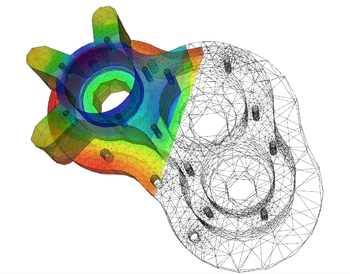
\includegraphics[height=3in]{img}
\vfill
\LARGE Brennan Reamer \\[.2in]
\texttt{reamerb1@wit.edu}\\
\texttt{December 2020}
\end{center}      
\end{titlepage}
\newpage
\tableofcontents
\newpage
\section{Numerical Methods of Solving Partial Differential Equations}
\subsection{Order of Error}
\begin{center}
$\ds \d{f}{x} = \lim_{x \to 0} \frac{f(x + \Delta x) - f(x)}{\Delta x}$ \hspace{1cm} $\implies$ \hspace{1cm}
$\ds \d{f}{x} \approx \frac{f(x + \Delta x) - f(x)}{\Delta x}$ \\ \vspace{5mm}
Taylor's Theorem: \phantom{aa} $ f(x + \Delta x) \approx f(x) + f'(x)\Delta x + \frac{f''(x) (\Delta x)^2}{2} + \frac{f'''(x) (\Delta x)^3}{3!} + \frac{f^{(4)}(x) (\Delta x)^4}{4!} + ...$ \\ \vspace{5mm}
Taylor's Theorem can be simplified to contain less terms by using the comprehensive error term $[\frac{f''(c) (\Delta x)^2}{2!}]$.\\ \vspace{5mm}
$ f(x + \Delta x) = f(x) + f'(x)\Delta x + ... + [\frac{f''(c) (\Delta x)^2}{2!}]$ \hspace{1cm} , \hspace{1cm} Where $c \in (x, x+ \Delta x)$\\ \vspace{5mm}
Error$(\Delta x) = \frac{M (\Delta x)^2}{2}$ \\ \vspace{5mm}
The equation can be rearranged to give us \\ \vspace{5mm}
$\boxed{f'(x) = \frac{f(x+ \Delta x) - f(x)}{\Delta x} + \frac{\textrm{Error}(\Delta x)}{\Delta x}}$ \\ \vspace{5mm}
$\frac{\textrm{Error}(\Delta x)}{\Delta x} \rightarrow \frac{M \Delta x}{2} \rightarrow O(\Delta x)$\\ \vspace{5mm}
In order to find the order of error, $O( \Delta x)$, of a given equation $f(x)$, you must multiply $f'(x)$ by the given $\Delta x$. \\
\end{center} \textbf{Mastery Check:} \\
Approximate $u'(x)$ using $u(x-h)$, $u(x)$, and $u(x+3h)$.\\ \\
 Rewrite $u(x-h)$, $u(x)$, and $u(x+3h)$ as their Taylor Series approximations:
\begin{eqnarray*}
u(x-h) &=& u(x) - u'(x)h + \frac{u''(x)h^2}{2} - \frac{u'''(x)h^3}{6} + \ldots \\ 
u(x+3h) &=& u(x) + u'(x)3h + \frac{u''(x)(3h)^2}{2} + \frac{u'''(x)(3h)^3}{6} +  \ldots \\  
u(x) &=& u(x)
\end{eqnarray*}
Figure out the coefficients:
\begin{eqnarray*}
\red{A}(\frac{u''(x)h^2}{2}) + \blue{B}(\frac{9u''(x)h^2}{2}) &=& 0 \longrightarrow \red{A}=-9\blue{B} \longrightarrow  \red{A}=-9, \blue{B}=1\\ 
\green{C}(u(x)) + \blue{B}(u(x))+\red{A}(u(x)) &=& 0 \longrightarrow \green{C} + 1 - 9 = 0 \longrightarrow \green{C} = 8\\
\red{A}(\frac{u'''(x)h^3}{6}) + \blue{B}(\frac{u'''(x)27h^3}{6}) &=& \frac{18u'''(x)h^3}{6} = 3u'''(x)h^3\\
\end{eqnarray*}
Combine the Taylor Series using the coefficients:
\begin{eqnarray*}
8u(x)+u(x+3h)-9u(x-h) &=& 0+3u'(x)h+9u'(x)h+0+...\\
u'(x) &=& \frac{8u(x)+u(x+3h)-9u(x-h)}{12h} + \frac{O(h^3)}{12h}\\
\end{eqnarray*}
Solving for $u'(x)$ and simplifying gives the final equation:
\begin{center}
\boxed{u'(x) = \frac{8u(x)+u(x+3h)-9u(x-h)}{12h} + O(h^2)}\\ 
\end{center}
\subsubsection{Error} The error is of order $h^2$. Order of error is directly proportional to $h^2$ (ie. $O(h^2) \propto h^2$). In the limit as $h^2 \to 0$, the error in the definition of a derivative also goes to 0. You cannot let $h^2$ become too small as your computer will be unable to calculate such small numbers. The \emph{machine epsilon} \label{machineepsilon} is the smallest number your computer can store and limits how small your calculations can reach.
\subsection{Neumann Stability}
Neumann Stability is a method of checking the stability of finite difference schemes. In order for the given scheme to be stable, the following condition must be met
\bea
|\lambda| &\leq& 1.
\eea
The problems generally begin by considering one Fourier mode of the solution:
\bea
e^{ikx_m} &=& u(t_j,x_m).
\eea
The following substitutions may then be made:
\bea
u_{j+1,m} = \lambda e^{ikx_m}, \hspace{5mm} u_{j,m+1} = e^{ik(x_m+\Delta x)}, \hspace{5mm} u_{j,m} = e^{ikx_m}, \hspace{5mm} u_{j,m-1} = e^{ik(x_m-\Delta x)}.
\eea
The given scheme may then be solved for the variable $\lambda$ and simplified to find if and when $|\lambda| \leq 1$.\\
If $|\lambda|$ is never $\leq 1$, then the scheme is unstable. If $|\lambda| \leq 1$ for some $a \leq \sigma = \frac{c\Delta t}{\Delta x} \leq b$, then the scheme is conditionally stable. If  $|\lambda|$ is always $\leq 1$, then the scheme is unconditionally stable.\\\\
\textbf{Mastery Check:}\\
Find the Neumann Stability for the following scheme.
\bea
u_{j+1,m} &=& \frac{1}{2}\sigma(\sigma-1)u_{j,m+1}-(\sigma^1-1)u_{j,m}+\frac{1}{2}\sigma(\sigma+1)u_{j,m-1}\\
\sigma &=& \frac{c\Delta t}{\Delta x}\\
u_t+cu_x &=& 0
\eea
Begin by setting the following substitutions:
\bea
u_{j+1,m} = \lambda e^{ikx_m}, \hspace{5mm} u_{j,m+1} = e^{ik(x_m+\Delta x)}, \hspace{5mm} u_{j,m} = e^{ikx_m}, \hspace{5mm} u_{j,m-1} = e^{ik(x_m-\Delta x)}.
\eea
Plug the substitutions into the scheme and solve for $\lambda$
\bea
\lambda e^{ikx_m} &=& \frac{1}{2}\sigma(\sigma-1)e^{ik(x_m+\Delta x)}-(\sigma^1-1)e^{ikx_m}+\frac{1}{2}\sigma(\sigma+1)e^{ik(x_m-\Delta x)}\\
\lambda &=& \sigma^2\cos(k\Delta x)-i\sigma\sin(k\Delta x)+1-\sigma^2\\
\left|\lambda\right| \leq 1 &\implies& \left|\lambda\right|^2 \leq 1\\
\left|\lambda\right|^2 &=& (1-\sigma^2(1-\cos(k\Delta x)))^2+\sigma^2\sin^2(k\Delta x)\\
\left|\lambda\right|^2 &=& (\sigma^2 - 1) \sigma^2 \cos^2(k\Delta x) + 2(1-\sigma^2) \sigma^2 \cos(k\Delta x) +
(1 - \sigma^2)^2 + \sigma^2
\eea
Set
\bea
g = \left|\lambda\right|^2 &,& \alpha = \cos(k\Delta x) \rightarrow \alpha \in [-1,1]
\eea
to make $g(\alpha)$ a quadratic function
\bea
g(\alpha) &=& (\sigma^2 - 1) \sigma^2 \alpha^2 + 2(1-\sigma^2) \sigma^2 \alpha +
(1 - \sigma^2)^2 + \sigma^2\\
\eea
which implies that the max occurs at
\bea
g'(\alpha) = 0 &\forall& \alpha \in [-1,1]\\
&\text{or at}&\\
\alpha &=& \pm 1.
\eea
We need to find: $|g| \leq 1$ with $\alpha \in [-1,1]$.\\
First, $g(1)$ and $g(-1)$ can be checked
\bea
g(1) &=& 1\\
g(-1) &=& \left(1-2\sigma^2\right)^2
\eea
Then, each case for the value of $|\sigma|$ can be checked.\\
Case 1: $|\sigma| > 1$
\bea
g(-1) &=& \left(1-2\left(|\sigma| > 1\right)^2\right)^2 \implies |g| > 1 \hspace{5mm} \forall \hspace{5mm} |\sigma| > 1
\eea
Unstable when $|\sigma| > 1$.\\
Case 2: $|\sigma| = 1$
\bea
g(\alpha) = 1 &\forall& \sigma = \pm 1
\eea
Stable when $|\sigma| = 1$.\\
Case 3:  $|\sigma| < 1$
\bea
g'(\alpha) = 0 = 2\left(\sigma^2-1\right)\sigma^2\alpha+2\left(1-\sigma^2\right)\sigma^2 &\implies& \text{Max occurs at } \alpha = 1\rightarrow g(1) = 1
\eea
Stable when $|\sigma| < 1$.\\
Summarizing the outcomes yields the solution:
\bea
\boxed{\text{Conditional Stability: }|\sigma| \leq 1}
\eea
 \subsection{The CFL Condition}
The CFL condition is a condition for convergence used when solving partial differential equations numerically using explicit time-dependent schemes.\\\\
Constant Wave Speed $c$:\\
The CFL condition typically has the following form
\bea
\sigma = &\frac{c\Delta t}{\Delta x}& \leq \sigma_{\text{max}}
\eea
where $c$ is the magnitude of the velocity of the function, $\Delta t$ is the time step, and $\Delta x$ is the spatial step. If an explicit scheme is used then typically $\sigma_{\text{max}} = 1$. Using an implicit scheme, larger values of $\sigma_{\text{max}}$ may be tolerated.\\\\
Upwind Scheme (Nonconstant Wave Speed $c$):\\
In order to overcome the sign restriction on a nonconstant wave speed two different schemes must be used, the forward difference scheme when the wave speed is negative and the backwards scheme when it is positive. The resulting scheme for nonconstant wave speeds is
\bea
u_{j+1,m} &=&\begin{cases}
-\sigma_{j,m}u_{j,m+1}+(\sigma_{j,m}+1)u_{j,m}, & c_{j,m} \leq 0\\
-(\sigma_{j,m}-1)u_{j,m}+\sigma_{j,m}u_{j,m-1}, & c_{j,m} > 0
\end{cases},
\eea
where
\bea
\sigma_{j,m} = c_{j,m}\frac{\Delta t}{\Delta x}, && c_{j,m} = c(t_j,x_m).
\eea
In order to remain stable, the step size must remain small and the CFL condition,
\bea
\frac{\Delta x}{\Delta t} \leq |c_{j,m}|,
\eea
 must be satisfied at each node.\\\\
\textbf{Mastery Check:}\\
Find the CFL condition of the following scheme.
\bea
u_t+cu_x &=& 0\\
u_{j+1,m} &=& Au_{j,m+3} + Bu_{j,m+2} + Cu_{j,m+1} + Du_{j,m} + Eu_{j,m-1}
\eea
The numerical domain of dependence can be graphed by observing where the variables of $u$ would land in the graph. For example, $u_{j,m+2}$ would be put at the point $(j,m+2)$ on the graph. The points can all be connected then to create the domain of dependence for the scheme.
\begin{figure} [H]
\begin{center}
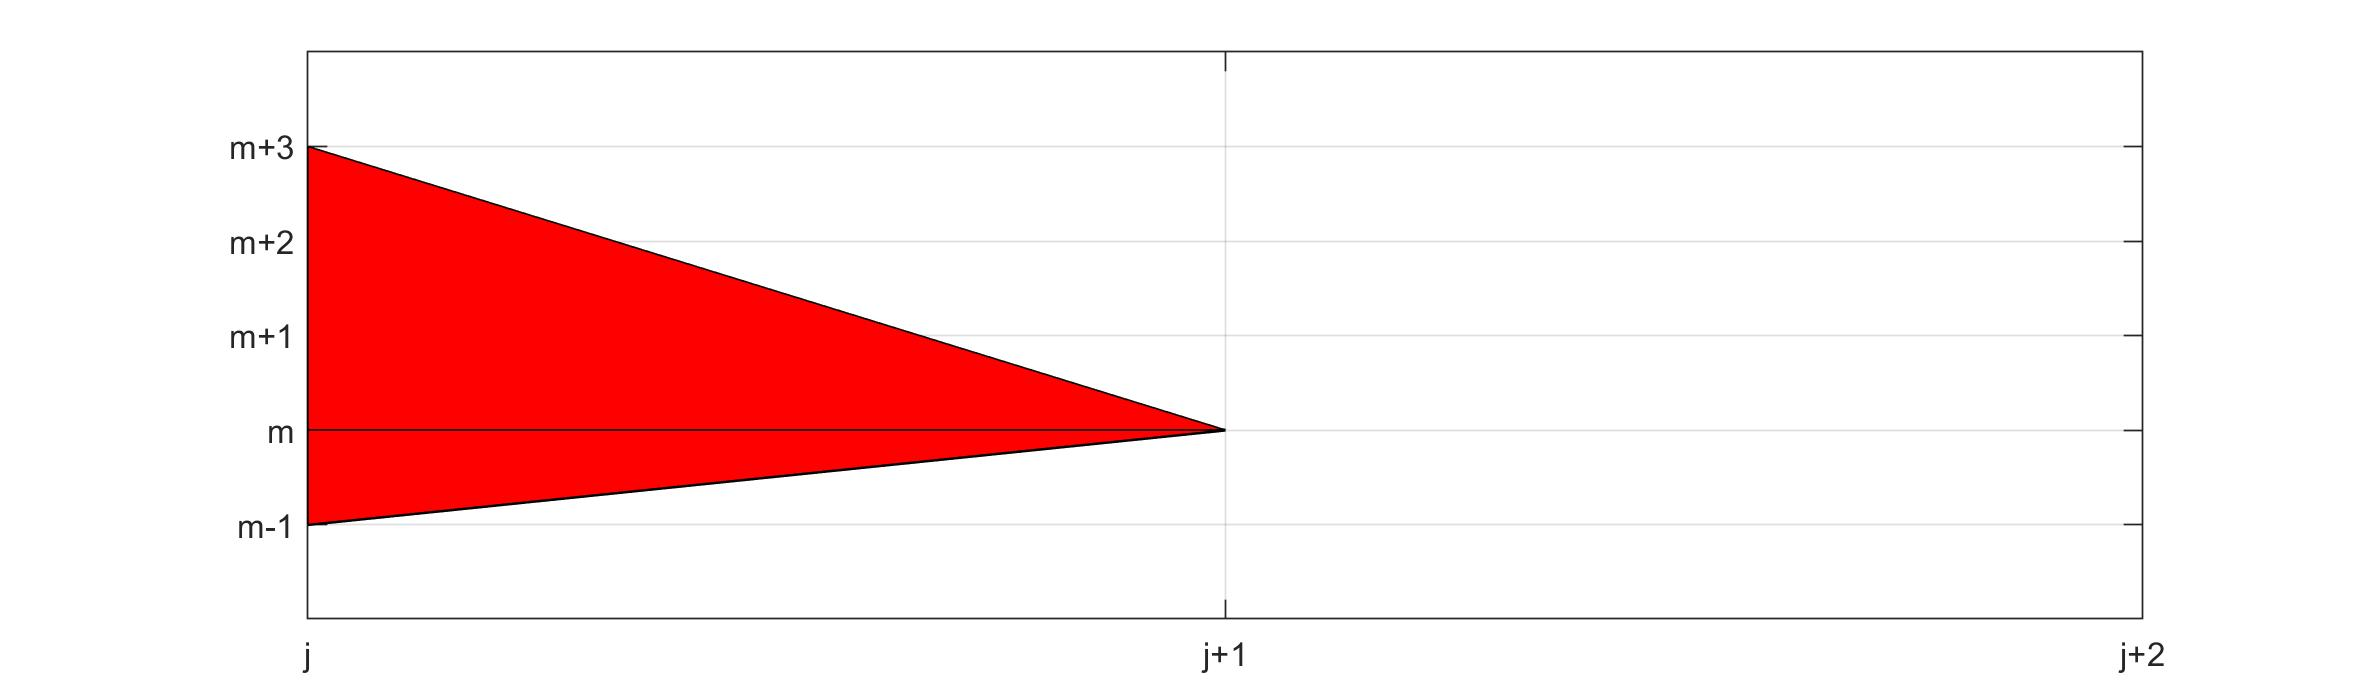
\includegraphics[width = 6.5 in, clip]{DomainOfDependence}
\caption{Numerical Domain of Dependence \label{fig:domain}}
\end{center}
\end{figure}
The CFL condtion states that the value must fall within the domain of dependence, shown above in Figure \ref{fig:domain}.
\bea
x_{m-1} \leq& x_m-ct_{j+1} &\leq x_{m+3}\\
-\Delta x \leq& -c\Delta t &\leq 3\Delta x
\eea
\begin{center}
\boxed{-1 \leq \sigma = \frac{-c\Delta t}{\Delta x} \leq 3}
\end{center}
\subsection{Implementing an Explicit Difference Method}
The explicit difference method uses the data from previous time steps to calculate the value at the current time step. A boundary value problem is a set of differential equations that have additional constraints, called boundary conditions. The boundary conditions used in the explicit difference method are often referred to as $\alpha$ and $\beta$. The boundary conditions are used to determine the values $u(t_j,x_0)$ and $u(t_j,x_n)$ on the boundary nodes. The remaining values in the solution matrix u are determined using the equation $u^{(j+1)} = Au^{(j)} + b^{(j)}$, where \\
\[
A = \begin{pmatrix}
		1-2\mu & \mu  & & &\\
		\mu & 1-2\mu & \mu & &\\
		& \mu & \ddots & \ddots &\\
		&& \ddots & \ddots & \mu\\
		&&& \mu & 1-2\mu
		\end{pmatrix}\\, \hspace{5mm}
b^{(j)} = \begin{pmatrix}
		\mu \alpha_j \\
		0\\
		0\\
		\vdots\\
		0\\
		\mu \beta_j
		\end{pmatrix}\\.
\]
\\
Note: Where $n = $ number of space steps $ =  \frac{l}{\Delta x}$: $A$ is an (n-1) x (n-1) matrix. $b$ is an (n-1) column matrix.\\\\
In order to avoid potential instability while using the explicit difference method, the following equation must be used
\bea
\Delta t \leq \frac{(\Delta x)^2}{2\gamma} \text{ .}\\
\eea
This condition makes the explicit difference method \emph{conditionally stable} because it must be met to maintain stability in the solution.\\\\
Example 5.4.\\
\bea
\gamma = 1, &\l = 1, &\Delta x = 0.1\\
\eea
\[ u(0,x) = f(x) =
\begin{cases}
-x, & \text{if $0 \leq x \leq \frac{1}{5}$} \\
x-\frac{2}{5}, & \text{if $\frac{1}{5} \leq x \leq \frac{7}{10}$} \\
1-x, & \text{if $\frac{7}{10} \leq x \leq 1$} \\
 \end{cases} \]
\begin{center}
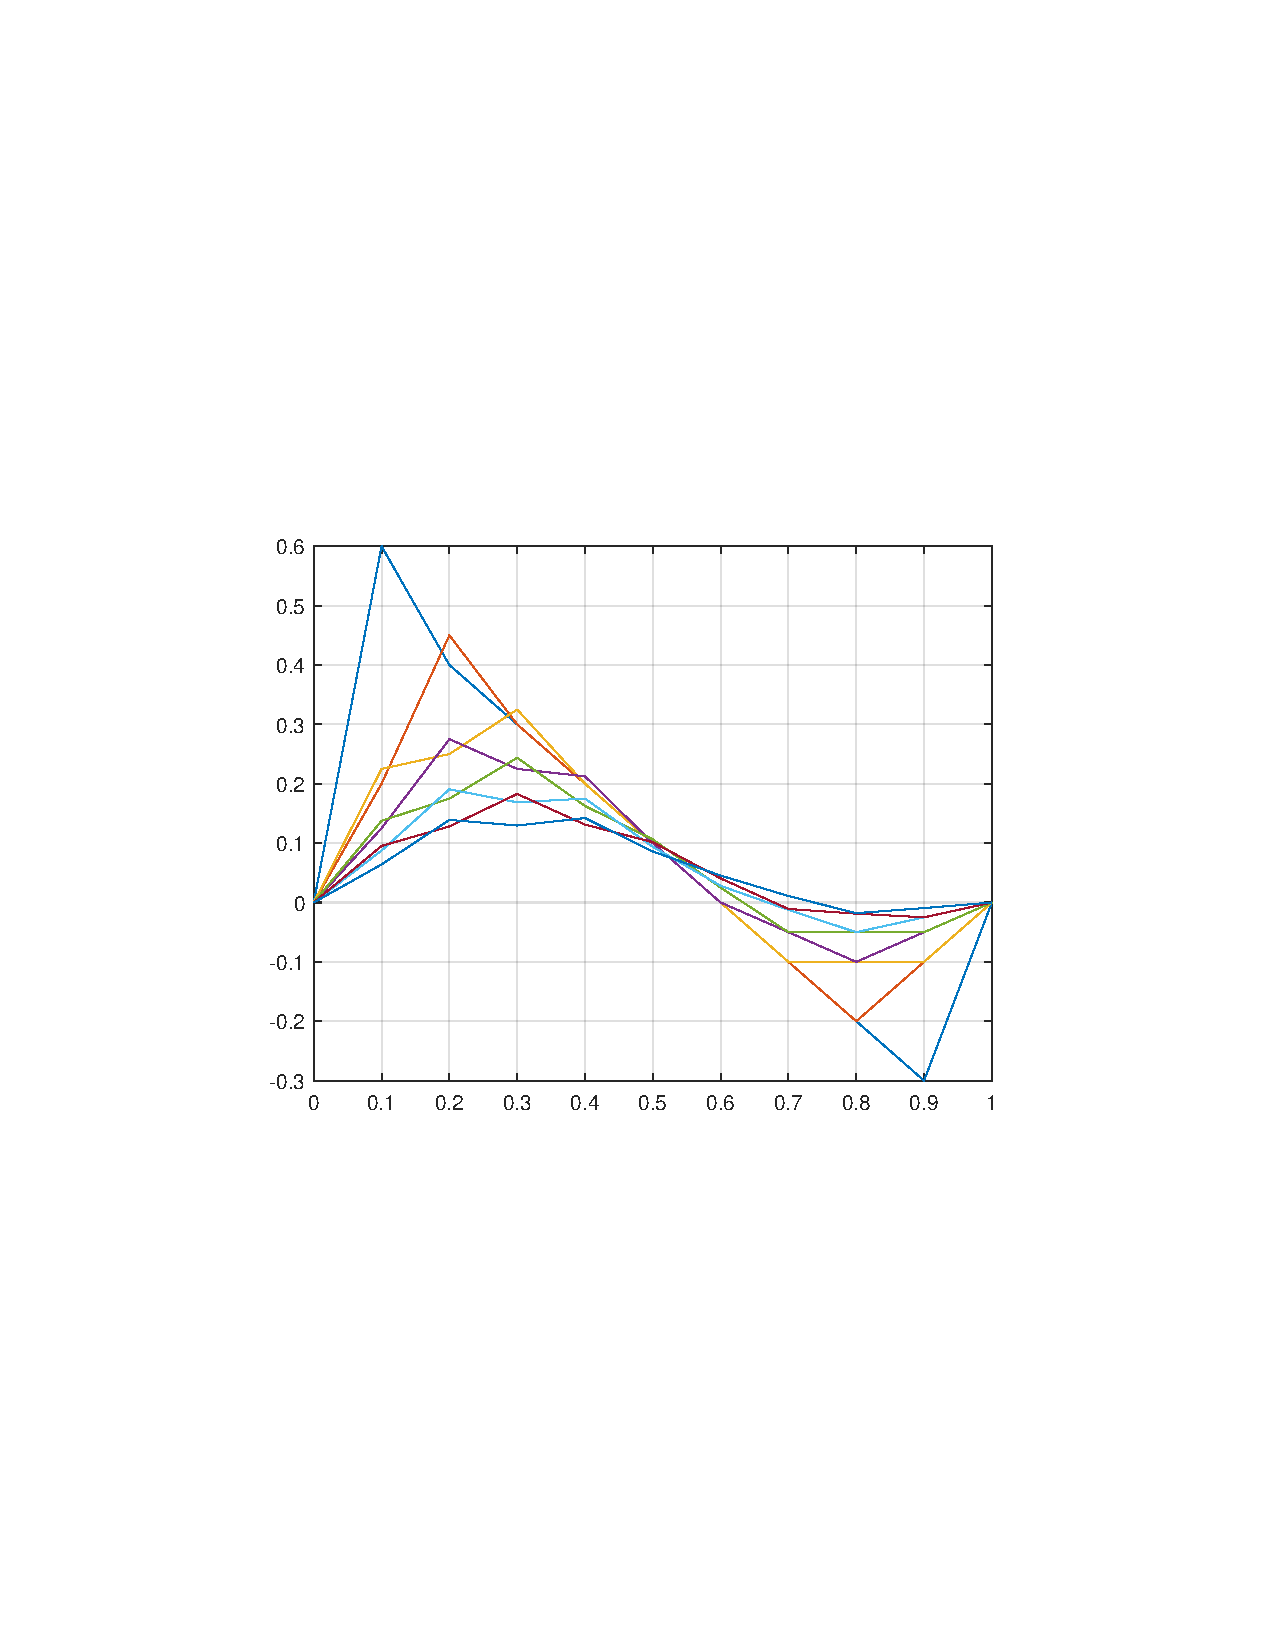
\includegraphics[height = 2.5 in, trim={4cm 9cm 4cm 9cm}, clip]{explicit_ex}
\end{center}

Mastery Problem:\\
\bea
u(t,0) &=& \cos(t)\\
u(t,1) &=& \sin(t)\\
\Delta x &=& 0.1\\
u_t &=& u_{xx}\\
\eea
\[ u(t,0) =
\begin{cases}
2 |x-\frac{1}{6}|, & \text{if $0 \leq x \leq \frac{1}{3}$} \\
0, & \text{if $\frac{1}{3} \leq x \leq \frac{2}{3}$} \\
\frac{1}{2}-3|x-\frac{5}{6}|, & \text{if $\frac{2}{3} \leq x \leq 1$} \\
 \end{cases} \]
Code:
\begin{verbatim}
%Inputs
L = 1;
gamma = 1; 					%diff(u,t) = gamma*diff(u,x,2);
delta_x = .1;
delta_t = delta_x^2/(2*gamma); 					% needs to be <= delta_x^2/2*gamma
t_end = 0.02;
mu = (gamma*delta_t)/(delta_x^2);
n = L/delta_x; 					% number of space steps
T = round(t_end/delta_t); 					% number of time steps
					% Creates Matrix A
A = full(gallery('tridiag', n-1, mu, 1-2*mu, mu)); 					% dimensions, diag: bottom, middle, upper
B = zeros(n-1,1); 					% Creates Matrix B
u = zeros(n+1, T); 					% Creates u-matrix
for z = 1:n-1
    x = z*delta_x;
    u(z+1, 1) = (0<=x<=(1/3)).*2*abs(x-(1/6)) + ((1/3<=x)&(x<=2/3)).*0 + 
						((2/3<=x)&(x<=1)).*(1/2)-3*abs(x-(5/6));
end
for j = 1:T
    B(1) = mu*alpha(j*delta_t);
    B(end) = mu*beta(j*delta_t);
    u(2:n,j+1) = (A*u(2:n,j))+B;
    u(1,j) = alpha(j*delta_t); 					% Adds in alpha to u-matrix
    u(end,j) = beta(j*delta_t); 					% Adds in beta to u-matrix
end
u(:,T+1) = []; 					% Removes the T+1'th column
figure
plot(linspace(0,L,n+1),u)
grid
function [a] = alpha(t) 					% Defines u(t,0)
    a = cos(t); 					% u(t,0)
end
function [b] = beta(t) 					% Defines u(t,L)
    b = sin(t); 					% u(t,L)
end
\end{verbatim}
Final Solution:\\
\begin{center}
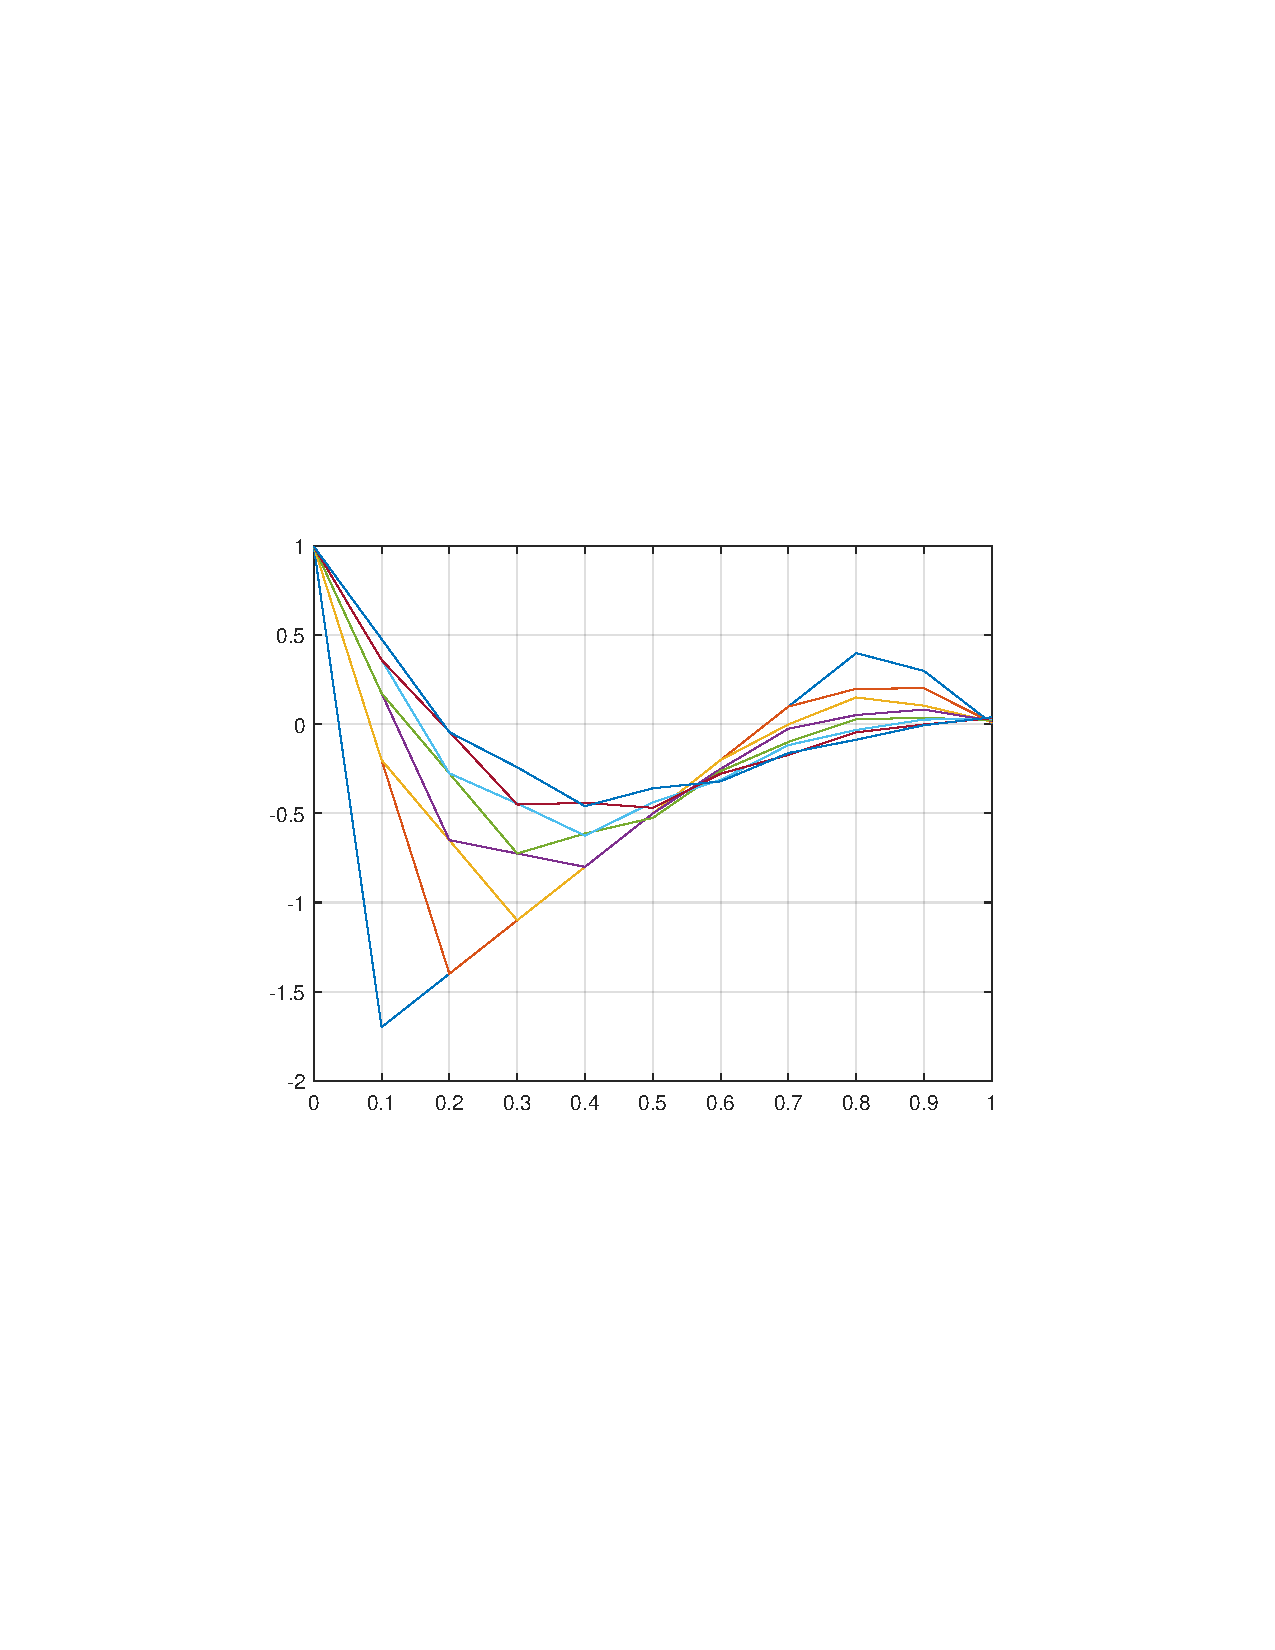
\includegraphics[height = 2.5 in, trim={4cm 9cm 4cm 9cm}, clip]{explicit}
\end{center}
\subsection{Implementing an Implicit Difference Method}
The Implicit Difference Method uses data from the current time step to calculate it's value. This method also has the boundary conditions $\alpha$ and $\beta$, which represent the solution function, $u$, at the designated time steps $t_0 = 0$ and $t_f = L$ . $\hat A$ is found from replacing $\mu$ with $-\mu$ in the Matrix $A$. The boundary conditions are used to determine the values $u(t_j,x_0)$ and $u(t_j,x_n)$ on the boundary nodes. The remaining values in the solution matrix $u$ are determined using the equation $u^{(j+1)} = \hat A^{-1} (u^{(j)} + b^{(j+1)})$, where \\
\[
\hat A = \begin{pmatrix}
		1+2\mu & -\mu  & & &\\
		-\mu & 1+2\mu & -\mu & &\\
		& -\mu & \ddots & \ddots &\\
		&& \ddots & \ddots & -\mu\\
		&&& -\mu & 1+2\mu
		\end{pmatrix}\\, \hspace{5mm}
b^{(j+1)} = \begin{pmatrix}
		\mu \alpha_{(j+1)} \\
		0\\
		0\\
		\vdots\\
		0\\
		\mu \beta_{(j+1)}
		\end{pmatrix}\\.
\]
\\
Note: Where $n = $ number of space steps $ =  \frac{l}{\Delta x}$: $\hat A$ is an (n-1) x (n-1) matrix. $b$ is an (n-1) column matrix.\\\\
While the explicit difference method was conditionally stable, the implicit difference method is \emph{unconditionally stable} as it does not require the restriction of the time step to maintain stability. This unconditional stability comes at the cost of having to invert the matrix $\hat A$.\\\\
Example 5.5.
\bea
\Delta x = 0.1\\
\Delta t = 0.01\\
t = 0.04\\
\eea
\begin{center}
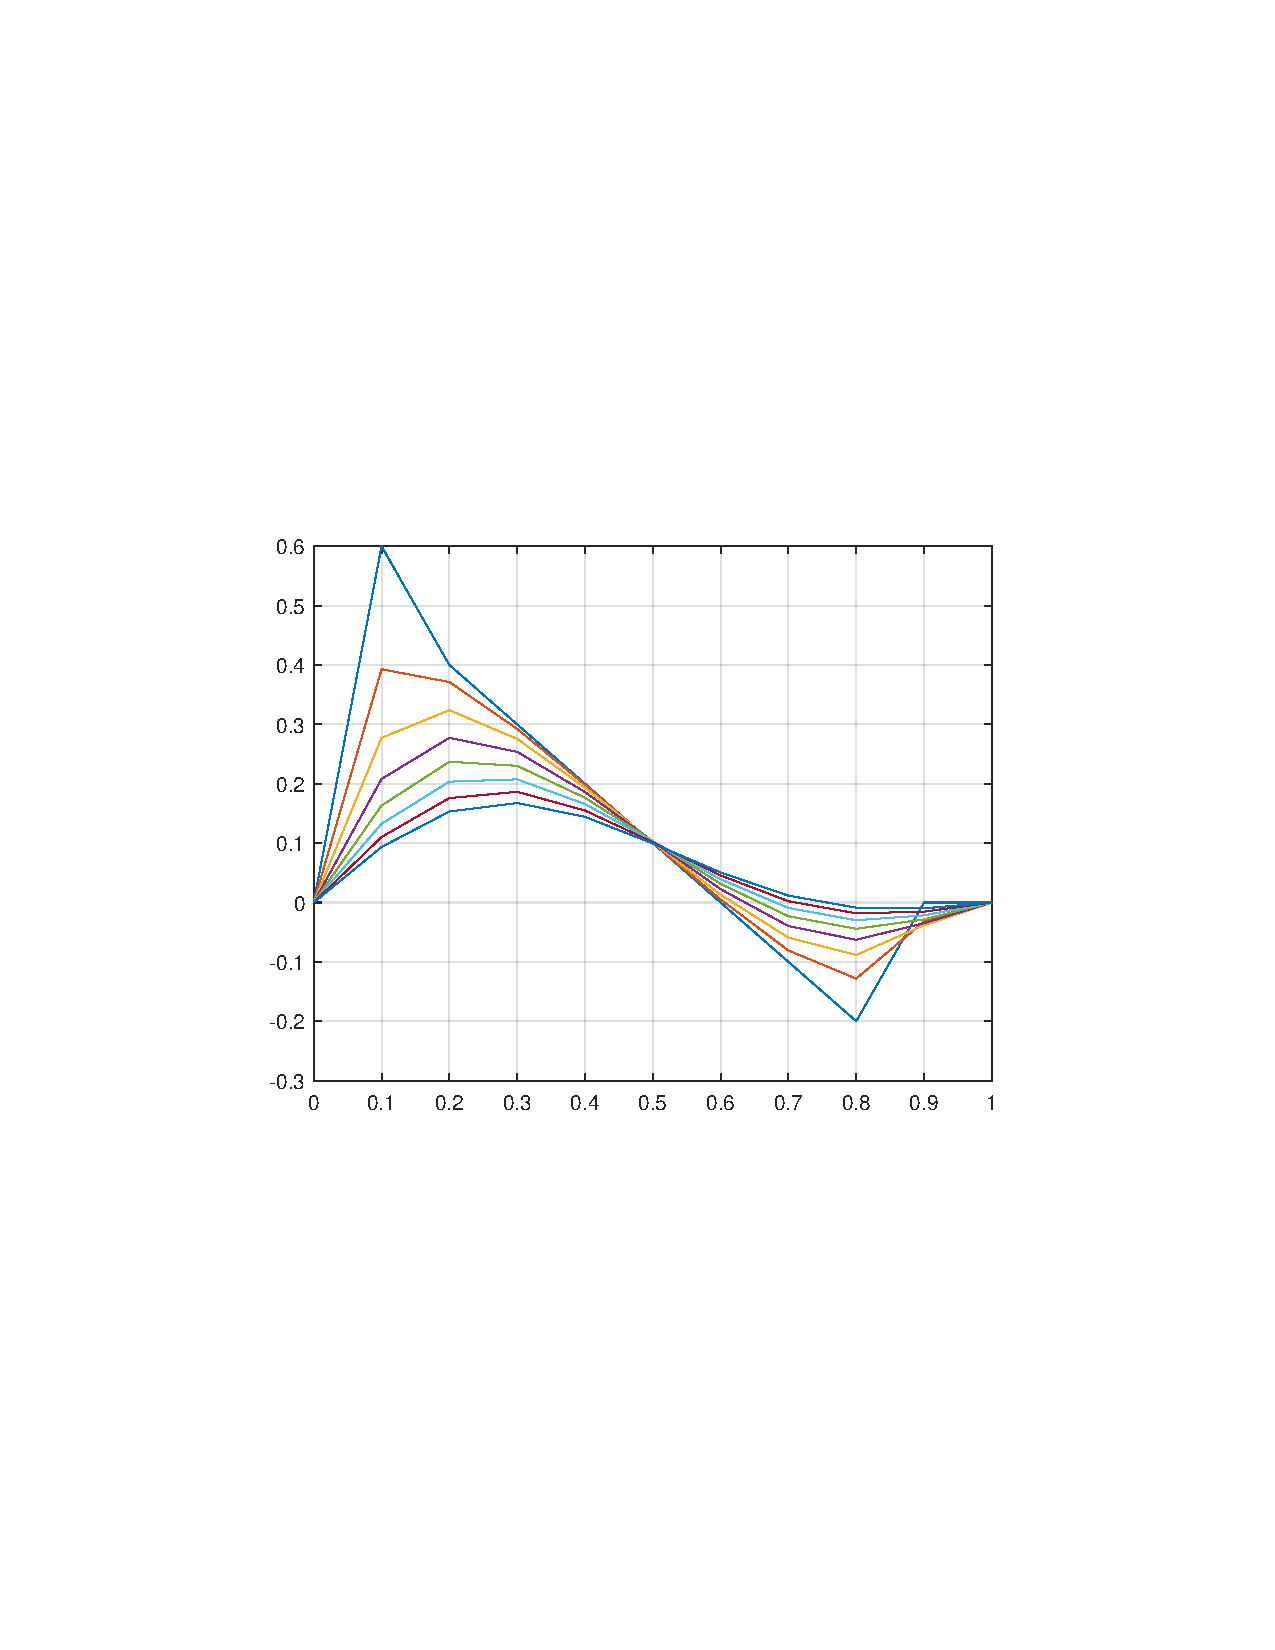
\includegraphics[height = 2.5 in, trim={4cm 9cm 4cm 9cm}, clip]{implicit_ex}
\end{center}
Mastery Problem:\\
\bea
u(0,x) &=& \cos(t)\\
u(1,x) &=& \sin(t)\\
\Delta x &=& 0.1\\
u_t &=& u_{xx}\\
\eea
\[ u(t,0) =
\begin{cases}
2 |x-\frac{1}{6}|, & \text{if $0 \leq x \leq \frac{1}{3}$} \\
0, & \text{if $\frac{1}{3} \leq x \leq \frac{2}{3}$} \\
\frac{1}{2}-3|x-\frac{5}{6}|, & \text{if $\frac{2}{3} \leq x \leq 1$} \\
\end{cases} \]
Code:
\begin{verbatim}
%Inputs
L = 1;
gamma = 1; %diff(u,t) = gamma*diff(u,x,2);
delta_x = .1;
delta_t = delta_x^2/(2*gamma); % needs to be <= delta_x^2/2*gamma
t_end = 0.02;
mu = (gamma*delta_t)/(delta_x^2);
n = L/delta_x; % number of space steps
T = round(t_end/delta_t); % number of time steps
% Creates Matrix A
A_hat = full(gallery('tridiag', n-1, -mu, 1+2*mu, -mu)); % dimensions, diag: bottom, middle, upper
B = zeros(n-1,1);% Creates Matrix B
u = zeros(n+1, T); % Creates u-matrix
for z = 1:n-2
    x = z*delta_x;
    u(z+1, 1) = (0<=x<=(1/3)).*2*abs(x-(1/6)) + ((1/3<=x)&(x<=2/3)).*0 + ((2/3<=x)&(x<=1)).*(1/2)-3*abs(x-(5/6));
end
for j = 1:T
    B(1) = mu*alpha((j+1)*delta_t);
    B(end) = mu*beta((j+1)*delta_t);
    u(2:n,j+1) = (inv(A_hat)*(u(2:n,j)+B));
    u(1,j) = alpha(j*delta_t); % Adds in alpha to u-matrix
    u(end,j) = beta(j*delta_t); % Adds in beta to u-matrix
end
u(:,T+1) = []; % Removes the T+1'th column
figure
plot(linspace(0,L,n+1),u)
grid
function [a] = alpha(t) % Defines u(0,x)
    a = cos(t);
end
function [b] = beta(t) % Defines u(L,x)
    b = sin(t);
end
\end{verbatim}
Final Solution:\\
\begin{center}
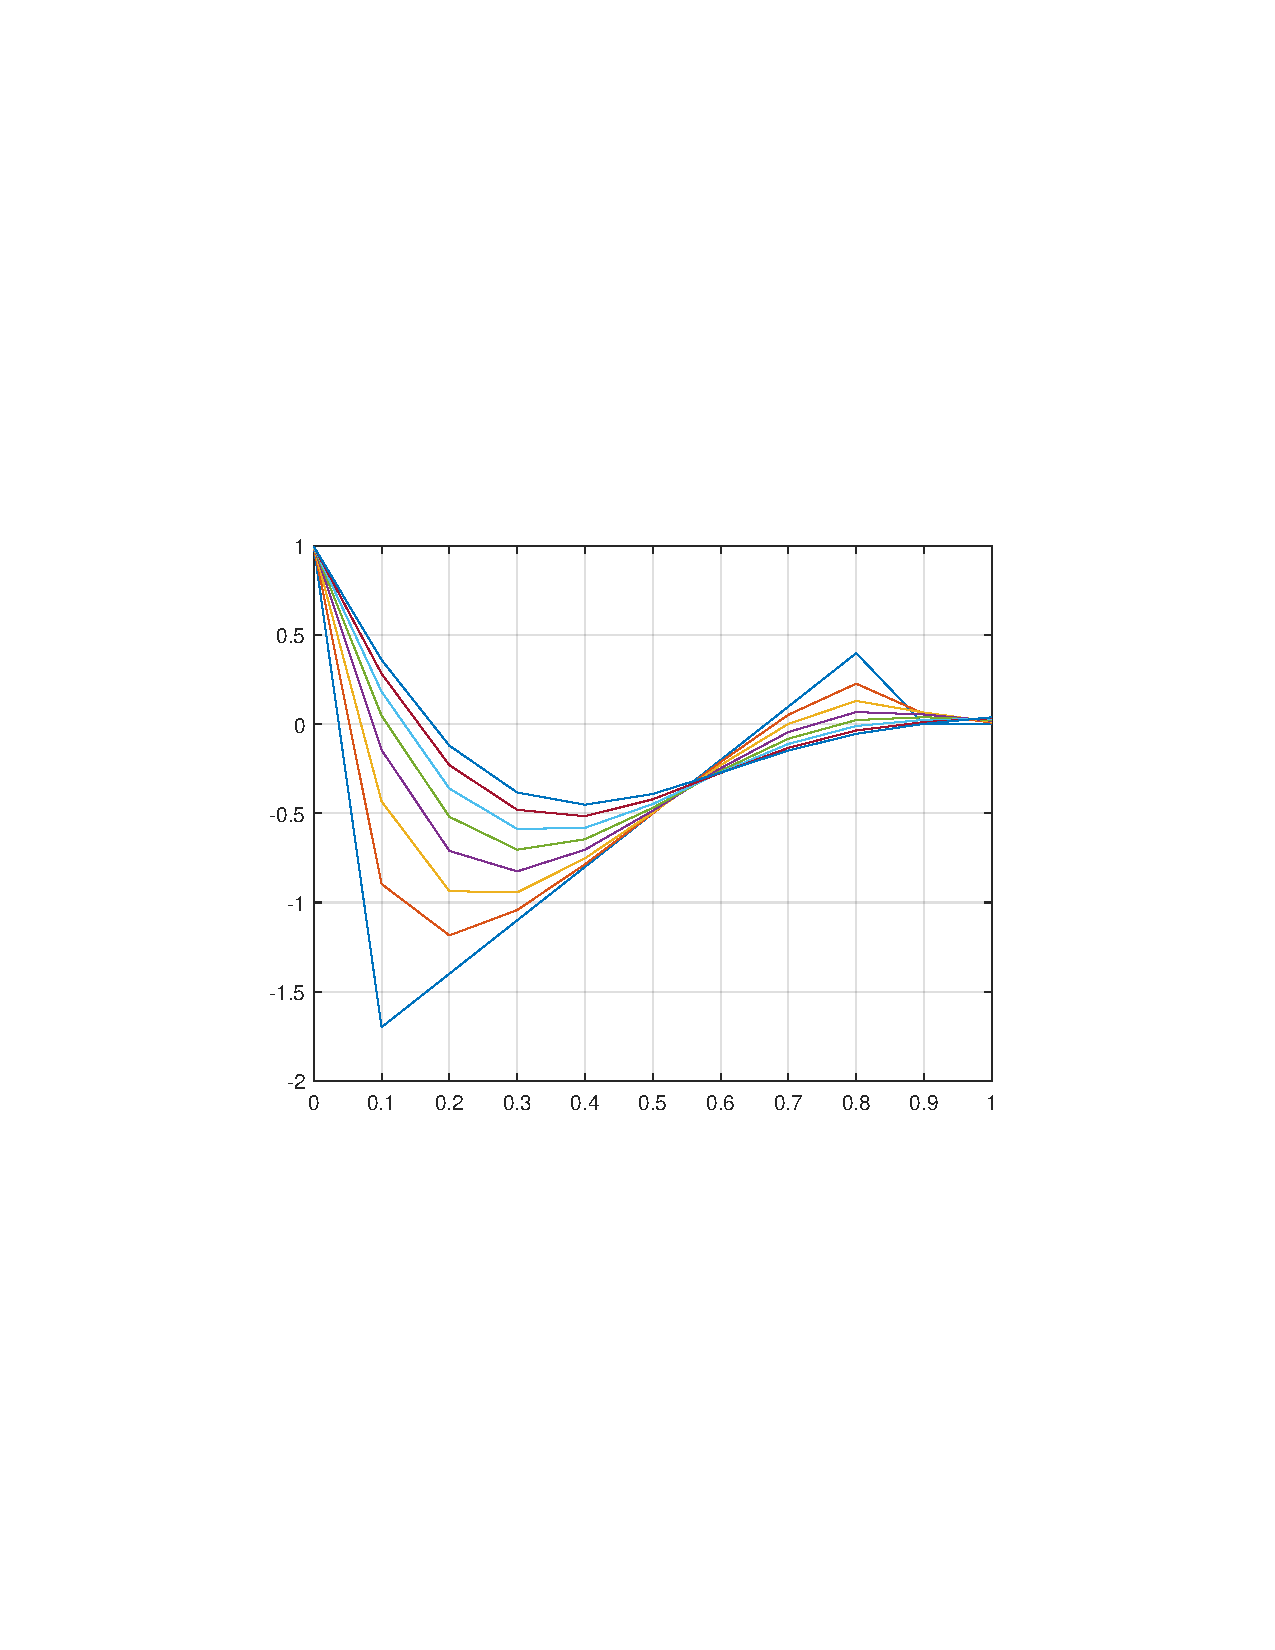
\includegraphics[height = 2.5 in, trim={4cm 9cm 4cm 9cm}, clip]{implicit}
\end{center}

\section{Method of Characteristics}
The Method of Characteristics is a technique for solving partial differential equations. The method uses the equation $\d{u}{t} = \pp{u}{t}\frac{dt}{dt} + \pp{u}{x}\frac{dx}{dt}$ to turn the partial differential equation into a series of ordinary differential equations. The ordinary differential equations can then be solved using the characteristic curves to find the solution to the given partial differential equation.
\subsection{Solving $u_t+cu_x +du = g(x)$ with $u(0,x)=f(x)$}
\bea
u(0,x)&=&f(x)\\
u_t+\red{c}u_x +\blue{d}u &=& g(x)\\
\eea
Rearrange equation to have all derivatives on one side.
\bea
u_t+\red{c}u_x&=& g(x)-\blue{d}u\\
\eea
Differentiate the function $u$ with respect to $t$ to create an equation that looks similar to what was given.
\bea
\pp{u}{t} &=& \pp{u}{t}\frac{dt}{dt} + \pp{u}{x}\frac{dx}{dt}\\
\pp{u}{t} &=& u_t + \frac{dx}{dt}u_x\\
\eea
Solve for the coefficient $\red{c}$ and integrate to find the constant $\xi$.
\bea
\frac{dx}{dt} &=& \red{c}\\
dx &=& \red{c}dt\\
x &=& \red{c}t + \xi\\
\xi &=& x-\red{c}t\\
\eea
Solve to find the equation h(t).
\bea
\d{u}{t} &=& u_t + \frac{dx}{dt}u_x\\
\d{u}{t} &=& u_t +\red{c}u_x\\
u_t +\red{c}u_x &=& g(x)-\blue{d}u\\
\frac{du}{dt} &=& g(x)-\blue{d}u\\
\eea
Integrate then find the constant of integration $k(\xi)$ using the initial condition $u(0,x)$.
Plug $k(\xi)$ back into the equation $h(t)$ to find the final solution.

\vspace{1cm}
\textbf{Mastery Problem:}
\bea
u_t-3u_x &=& 12\\
u(0,x) &=& \frac{\arctan(x)}{x^2+1}\\
\eea
Differentiate the function $u$ with respect to $t$ to create an equation that looks similar to what was given.
\bea
\pp{u}{t} &=& \pp{u}{t}\frac{dt}{dt} + \pp{u}{x}\frac{dx}{dt}\\
\pp{u}{t} &=& u_t + \frac{dx}{dt}u_x\\
\eea
Solve for the coefficients and integrate to find the constant $\xi$.
\bea
\frac{dx}{dt} &=& -3\\
dx &=& -3dt\\
x &=& -3t + \xi\\
\xi &=& x+3t\\
\eea
Solve to find the equation h(t).
\bea
\pp{u}{t} &=& u_t + \frac{dx}{dt}u_x\\
\pp{u}{t} &=& u_t -3u_x\\
u_t -3u_x &=& 12\\
\frac{du}{dt} &=& 12\\
\int du &=& \int{12}dt\\
h(t) &=& 12t+k(\xi)\\
\eea
Find $k(\xi)$ using the initial condition $u(0,x)$.
\bea
k(\xi) \hspace{2mm} = \hspace{2mm} u(0,\xi) &=& \frac{\arctan(x+3t)}{(x+3t)^2+1}\\
\eea
Plug $k(\xi)$ back into the equation $h(t)$ to find the final solution.
\begin{center}
\boxed{h = 12t + \frac{\arctan(x+3t)}{(x+3t)^2+1}}
\end{center}

\subsection{Solving the linear transport equation with polynomial coefficients}
\bea
u_t + c(x)u_x &=& 0\\
u(0,x) &=& f(x)\\\\
\d{x}{t} &=& c(x)\\
\xi &=& x(0)\\
\int_{\xi}^{x}{\frac{1}{c(x)}\,dx} &=& \int_{0}^{t}{1\,dt}\\
\eea
Solve for $\xi$ in terms of $x$ and $t$. Then plug into initial function.
\bea
u(0,x) &=& f(x)\\
u(t,x) &=& f(\xi)\\
\eea
Check by plugging $0$ in for $t$ in the equation $f(\xi)$. It should equal the original function $f(x)$.
\bea
f(x(0)) &=& u(0,x)\\
\eea
\textbf{Mastery Check:}\\
\bea
u_t + (x-5)(x-1)(t+6)u_x &=& 0\\
u(0,x) &=& \frac{3\cos(x)}{x^2+6}\\
\eea
Determine $\d{x}{t}$ and integrate to solve for $\xi$.
\bea
\d{x}{t} &=& (x-5)(x-1)(t+6)\\
\int_{\xi}^{x}{\frac{1}{(x-5)(x-1)}}{dx} &=& \int_{0}^{t}{t+6}{dt}\\
\frac{1}{4} \left(\ln\left|\frac{x-5}{x-1}\right| - \ln\left|\frac{\xi-5}{\xi-1}\right|\right) &=& \frac{1}{2}t^2+6t\\
\left(\frac{x-5}{x-1}\right)\left(\frac{\xi-1}{\xi-5}\right) &=& e^{2t^2+24t}\\
\xi &=& \frac{1-5\left(\frac{x-1}{x-5}\right)\left(e^{2t^2+24t}\right)}{1-\left(\frac{x-1}{x-5}\right)\left(e^{2t^2+24t}\right)}\\
\eea
Plug $\xi$ in for $x$ in $u(0,x)$ to find the solution equation $u(t,x)$.
\bea
u(t,\xi) &=& \frac{3\cos(\xi)}{\xi^2+6}\\
\eea
\begin{center}
\boxed{u(t,x) = \frac{3\cos(\frac{1-5\frac{x-1}{x-5}e^{2t^2+24t}}{1-\frac{x-1}{x-5}e^{2t^2+24t}})}{(\frac{1-5\frac{x-1}{x-5}e^{2t^2+24t}}{1-\frac{x-1}{x-5}e^{2t^2+24t}})^2+6}}
\end{center}
\subsection{Solving first order nonlinear PDEs using the method of characteristics}
\bea
u_t + g(u)u_x &=& 0\\
u(0,x) &=& f(x)\\
\eea
Solve for $x$ by plugging $u(0,\xi)$  into $g(u)$ because $u$ is constant along all time $t$, and integrating.
\bea
\d{x}{t} &=& g(u)\\
\d{x}{t} &=&g( u(0,\xi)) = g(f(\xi))\\
\int_{\xi}^{x}{\,dx} &=& \int_{0}^{t}{g(f(\xi))\,dt}\\
x &=& g(f(\xi))t+\xi\\
\eea
Check for a rarefaction or a shock in the characteristic curves and resolve them if there is one using the methods listed in the next sections. A suitable conservation law (ie. Conservation of mass, energy, etc.) in terms of $g(u)$ would be needed if there is a shock. A conservation law ensures that the solution follows the laws of physics and provides us with a realistic solution.\\\\
\textbf{Mastery Check:}\\
\bea
u_t+(u-3)^3u_x &=& 0\\
u(0,x) &=& \begin{cases}
2, & x<1\\
4, & x>1\\
\end{cases}\eea
\bea
\d{x}{t} &=& (u-3)^3\\
x &=& (u(0,\xi)-3)^3t+\xi\\
x &=& \begin{cases}
\xi-t, & \xi<1\\
\xi+t & \xi>1\\
\end{cases}
\eea
The rarefaction begins at $\xi = 1$, or $(0,1)$.
\bea
m &=& \frac{x-1}{t-0} = \frac{x-1}{t}\\
(u-3)^3 &=& \frac{x-1}{t}\\
u &=& \sqrt[3]{\frac{x-1}{t}}+3\\
\eea
Final Solution:
\begin{center}
\boxed{
u(t,x) = \begin{cases}
2, & x<1-t\\
\sqrt[3]{\frac{x-1}{t}}+3, & 1-t<x<1+t\\
4, & x>1+t\\
\end{cases}
}
\end{center}
\begin{figure}[H]
\begin{center}
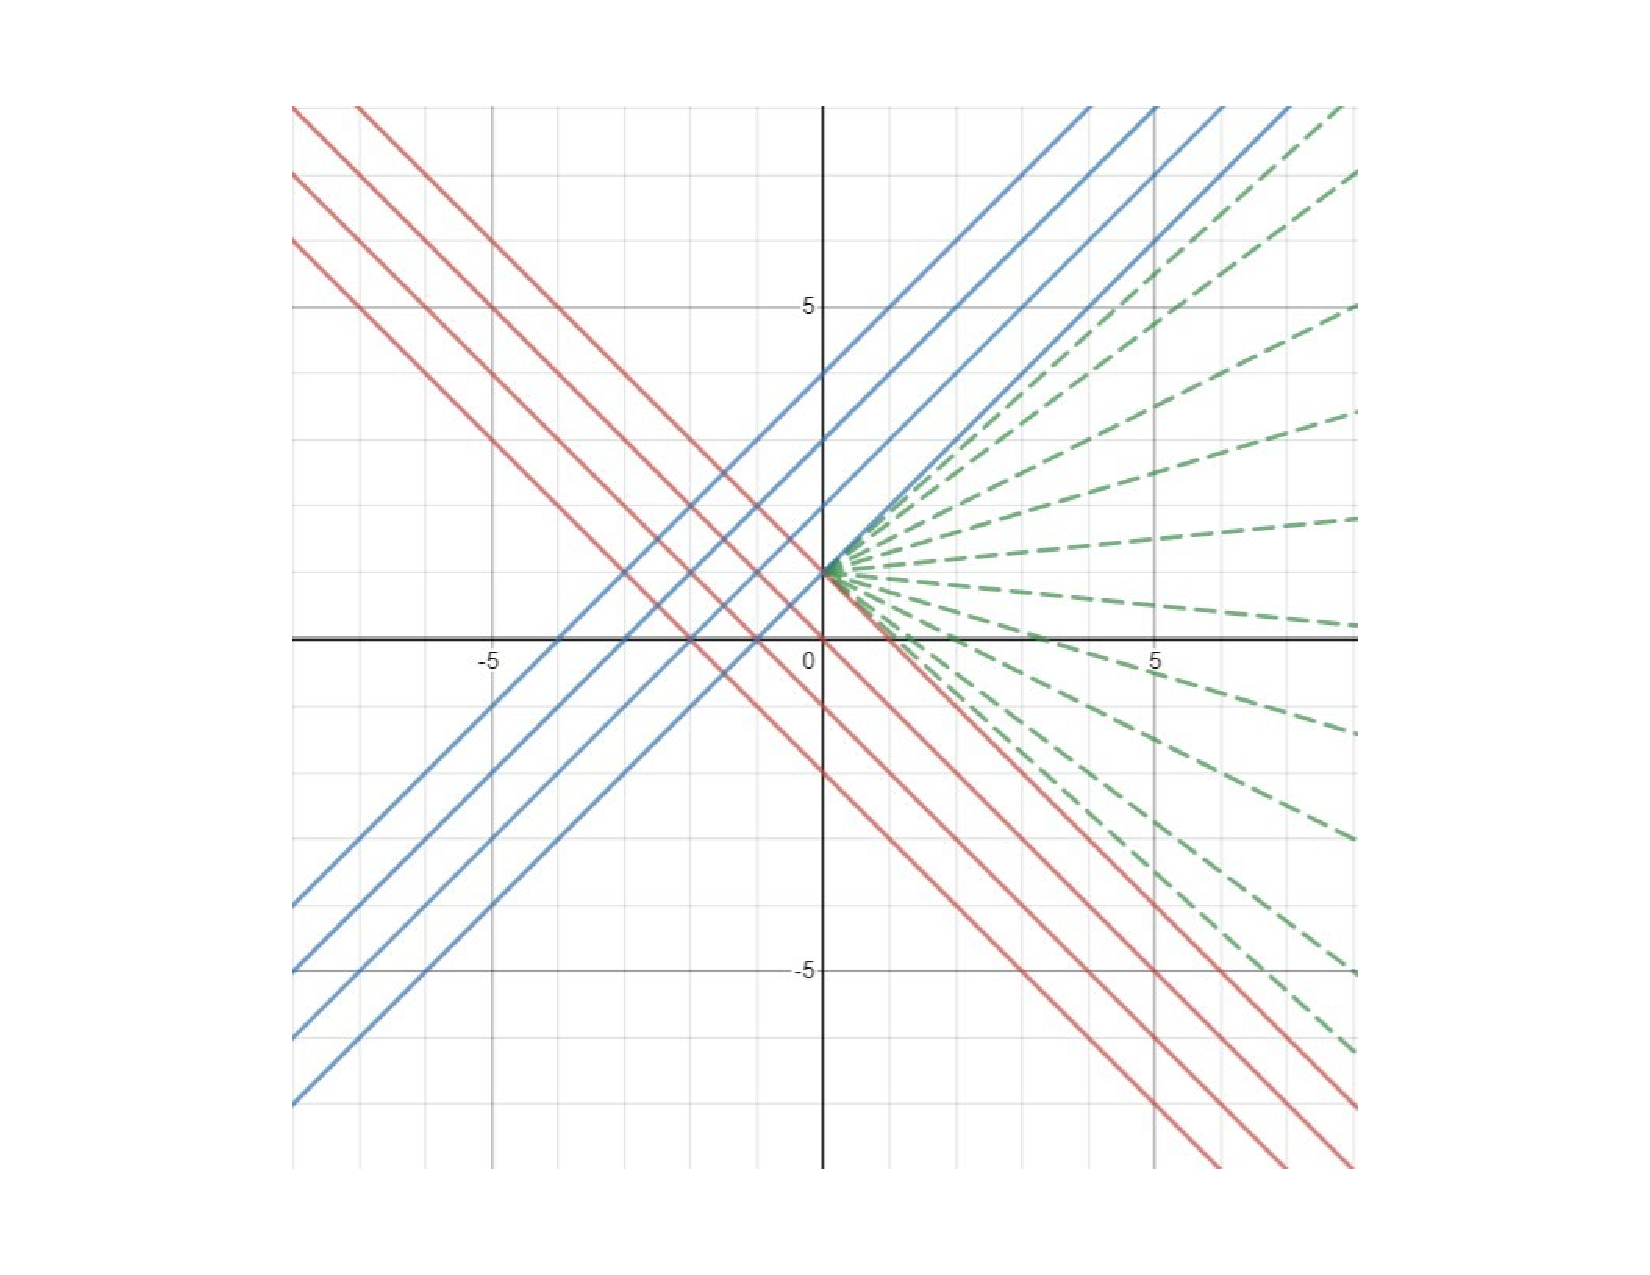
\includegraphics[height = 3 in, trim={4cm 4cm 4cm 4cm}, clip]{nonlinear}
\end{center}
\caption{Graph showing the \green{rarefaction} region. \label{fig:example}}
\end{figure}
\subsection{Shocks}
A shock occurs when the characteristic curves intersect with each other. The time a shock begins can be found using
\bea
t_* &\defeq& \mbox{min}\left\{-\frac{1}{f'(x)}\biggr|f'(x)<0\right\}.
\eea
Shocks need to be resolved because a shock means that there are multiple values for the function at the points in the shock region. Resolving the shock using the method below creates a line $\sigma(t)$ that separates the conflicting characteristic curves and resolves the problem of having multiple values for each point in the region.\\
\bea
u_t+g(u)u_x &=& 0\\
u(0,x) &=& f(x)\\
\text{Conservation of Mass:}\\
T = u &,& X = \frac{u^2}{2}\\
\eea
Solve for the Shock line $\sigma(t)$ by using the conservation law given.
\bea
\d{x}{t} &=& g(u(0,x))\\
x&\longrightarrow& \sigma\\
\d{\sigma}{t} &=& \frac{X^{+}-X^{-}}{T^{+}-T^{-}} = \frac{\frac{(g(u^{+}))^2}{2}-\frac{(g(u^{-}))^2}{2}}{g(u^{+})-g(u^{-})}\\
\eea
Solve and integrate to find $\sigma(t)$ using the initial conditions and the characteristic curves of $f(x)$ to figure out the constant of integration.\\\\
\textbf{Mastery Check:}\\
\bea
u_t+uu_x&=&0\\
u(0,x)&=& \begin{cases}
\red{0,} & \red{x<-1}\\
x, & -1<x<0\\
\blue{3,} & \blue{0<x}\\
\end{cases}\\
\text{Conservation of Mass:}\\
T = u &,& X = \frac{u^2}{2}\\
\eea
Shock:\\
Solve for the Shock line $\sigma(t)$ by using the conservation law given.
\bea
\d{x}{t} &=& u(0,x)\\
\d{\sigma}{t} &=& \frac{\frac{(u^{+})^2}{2}-\frac{(u^{-})^2}{2}}{u^{+}-u^{-}}\\
u^{+} &=& \xi = \frac{\sigma}{t+1}\\
\d{\sigma}{t} &=& \frac{\frac{\left(\frac{\sigma}{t+1}\right)^2}{2}-0}{\sigma-0} = \frac{\sigma}{2(t+1)^2}\\
\eea
The Shock begins at $(0,-1)$ based off of the intitial conditions and by looking at the graph (Figure$~\ref{fig:rarefaction}$).
\bea
\sigma(0) &=& -1\\
\purple{\sigma(t)} &=& -e^{-\frac{1}{2(t+1)}}\\
\eea
Rarefaction:\\
An equation needs to be found that can reflect the slope of each line in a rarefaction fan to fill in the empty space in the graph.\\
The rarefaction begins at $(0,0)$.\\
\bea
m &=& \frac{x-0}{t-0} = \frac{x}{t}\\
\eea
Final Solution:
\begin{center}
\boxed{
u(t,x) = \begin{cases}
\red{0,} & x<\purple{ -e^{-\frac{1}{2(t+1)}}}\\
x, & \purple{ -e^{-\frac{1}{2(t+1)}}}<x<0\\
\green{\frac{x}{t},} & 0<x<3t\\
\blue{3,} & x>3t\\
\end{cases}
}\end{center}
\begin{figure}[H]
\begin{center}
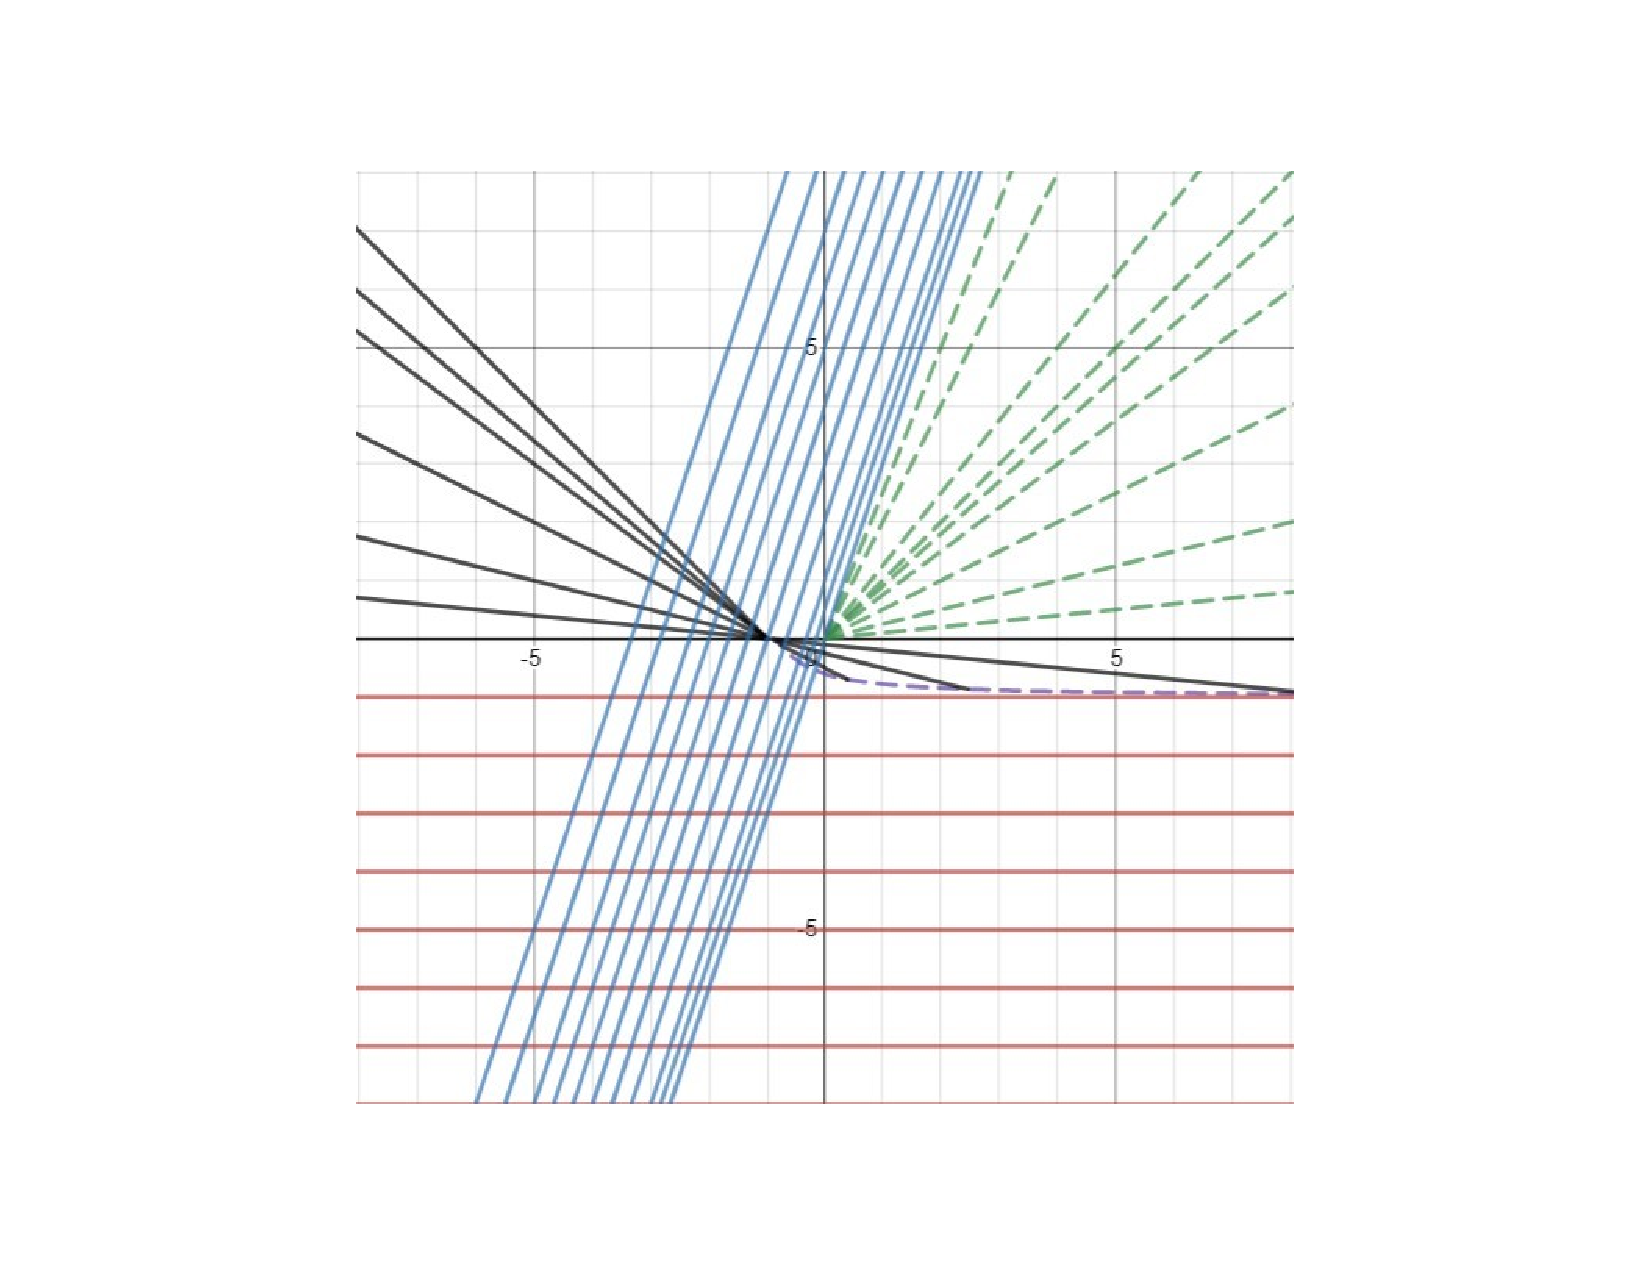
\includegraphics[height = 2.5 in, trim={4cm 4cm 4cm 4cm}, clip]{RarefactionShock}
\end{center}
\caption{Graph showing the \purple{shock} and \green{rarefaction} regions. \label{fig:rarefaction}}
\end{figure}

\subsection{Rarefaction Waves}
A rarefaction occurs whenever there are no values for the function in a region of points. On a graph of characteristic curves, this looks like a region of blank space between characteristic curves. To resolve a characteristic curve, an equation must be found to reflect the slope of each line in a rarefaction fan to fill in the region of empty space. The green lines in Figure$~\ref{fig:rarefaction}$ represent the lines of the rarefaction fan filling in the rarefaction region between the blue characteristic curves and the black characteristic curves.
\bea
u_t+g(u)u_x &=& 0\\
u(0,x) &=& f(x)\\
\eea
Solve for the slope of the rarefaction lines, where $(t_{0},x_{0})$ is the initial point where the rarefaction begins, by knowing that any point in the rarefaction region $(t,x)$ will have a slope of:\\
\bea
m &=& \frac{x-x_{0}}{t-t_{0}}\\
\eea
Set
\bea
g(u) &=& m\\
\eea
And solve for u to find the function $h(t,x)$ that will be the value of $u(t,x)$ inside the bounds of the rarefaction region.\\
\bea
u(t,x) &=& h(t,x)\\
\eea
\textbf{Mastery Check:}\\
\bea
u_t+uu_x&=&0\\
u(0,x)&=& \begin{cases}
\red{0,} & \red{x<-1}\\
x, & -1<x<0\\
\blue{3,} & \blue{0<x}\\
\end{cases}\\
\text{Conservation of Mass:}\\
T = u &,& X = \frac{u^2}{2}\\
\eea
Shock:\\
Solve for the Shock line $\sigma(t)$ by using the conservation law given.
\bea
\d{x}{t} &=& u(0,x)\\
\d{\sigma}{t} &=& \frac{\frac{(u^{+})^2}{2}-\frac{(u^{-})^2}{2}}{u^{+}-u^{-}}\\
u^{+} &=& \xi = \frac{\sigma}{t+1}\\
\d{\sigma}{t} &=& \frac{\frac{\left(\frac{\sigma}{t+1}\right)^2}{2}-0}{\sigma-0} = \frac{\sigma}{2(t+1)^2}\\
\eea
The Shock begins at $(0,-1)$ based off of the intitial conditions and by looking at the graph (Figure$~\ref{fig:rarefaction}$).
\bea
\sigma(0) &=& -1\\
\purple{\sigma(t)} &=& -e^{-\frac{1}{2(t+1)}}\\
\eea
Rarefaction:\\
An equation needs to be found that can reflect the slope of each line in a rarefaction fan to fill in the empty space in the graph.\\
The rarefaction begins at $(0,0)$.\\
\bea
m &=& \frac{x-0}{t-0} = \frac{x}{t}\\
\eea
Final Solution:
\begin{center}
\boxed{
u(t,x) = \begin{cases}
\red{0,} & x<\purple{ -e^{-\frac{1}{2(t+1)}}}\\
x, & \purple{ -e^{-\frac{1}{2(t+1)}}}<x<0\\
\green{\frac{x}{t},} & 0<x<3t\\
\blue{3,} & x>3t\\
\end{cases}
}\end{center}
Refer to Figure$~\ref{fig:rarefaction}$ for a graph of the characteristic curves of the final solution.

\section{Fourier Series}
Fourier Series are able to represent any function as an infinite series of sines and cosines. Many modern technologies, such as phones, televisions, and computers, were made using Fourier Series. The Gibbs Phenomenon is an overshoot that occurs at the point of a jump discontinuity in the Fourier Series representation of a function. The region of overshoot becomes narrower as the number of terms increases, but the amount of overshoot relative to the rest of the approximation remains the same.
\subsection{Real Fourier Series}
The Fourier Series for a function $f(x)$ on an interval $[-L,L]$ is
\begin{eqnarray}
f(x) &\sim& \frac{a_0}{2} + \sum_{k=1}^{\infty}{a_k\cos\left(\frac{k\pi x}{L}\right)+b_k\sin\left(\frac{k\pi x}{L}\right)}
\end{eqnarray}
The variables $a_0$, $a_k$, and $b_k$ can be found using the following equations
\begin{eqnarray}
a_0 &=& \frac{1}{L}\int_{-L}^{L}{f(x)}dx\\
a_k &=& \frac{1}{L}\int_{-L}^{L}{f(x)\cos\left(\frac{k\pi x}{L}\right)}dx\\
b_k &=& \frac{1}{L}\int_{-L}^{L}{f(x)\sin\left(\frac{k\pi x}{L}\right)}dx
\end{eqnarray}
The variables solved for using the above equations can then be inserted into the Fourier Series equation to find the Fourier Series for the function $f(x)$.\\\\
\textbf{Mastery Check:}\\
\bea
f(x) &=& |x-2|
\eea
on the interval $[-5,5]$.\\\\
Calculate the variable $a_0$ using equation (2) and simplify.
\bea
a_0 &=& \frac{1}{5}\int_{-5}^{5}{|x-2|}dx\\
a_0 &=& \frac{29}{5}\\
\eea
Calculate the variable $a_k$ using equation (3) and simplify.
\bea
a_k &=& \frac{1}{5}\int_{-5}^{5}{|x-2|\cos\left(\frac{k\pi x}{5}\right)}dx\\
a_k &=& \frac{10(-1)^k-10\cos\left(\frac{2\pi k}{5}\right)}{\pi^2k^2}\\
\eea
Calculate the variable $b_k$ using equation (4) and simplify.
\bea
b_k &=& \frac{1}{5}\int_{-5}^{5}{|x-2|\sin\left(\frac{k\pi x}{5}\right)}dx\\
b_k &=& \frac{4\pi k(-1)^k-10\sin\left(\frac{2\pi k}{5}\right)}{\pi^2k^2}\\
\eea
Plug the values for the variables $a_0$, $a_k$, and $b_k$ back into equation (1) to find the solution.
\begin{center}\boxed{
f(x) \sim 2.9 + \sum_{k=1}^{\infty}{\frac{10(-1)^k-10\cos\left(\frac{2\pi k}{5}\right)}{\pi^2k^2}\cos\left(\frac{k\pi x}{5}\right)+\frac{4\pi k(-1)^k-10\sin\left(\frac{2\pi k}{5}\right)}{\pi^2k^2}\sin\left(\frac{k\pi x}{5}\right)}
}\end{center}
\subsection{Complex Fourier Series}
The complex Fourier Series for a function $f(x)$ is
\bea
f(x) &\sim& C_0+\sum_{k=-\infty}^{\infty}{C_ke^{ikx}}
\eea
The following formulas are often used to simplify f(x) before calculating $C_k$ to make the math simpler.
\bea
e^{i\pi} &=& -1\\
e^{ikx} &=& \cos(kx)+i\sin(kx)\\
e^{-ikx} &=& \cos(kx)-i\sin(kx)\\
\cos(kx) &=& \frac{e^{ikx}+e^{-ikx}}{2}\\
\sin(kx) &=& \frac{e^{ikx}-e^{-ikx}}{2i}\\
a_k &=& C_k+C_{-k}\\
b_k &=& i\left(C_k-C_{-k}\right)\\
C_k &=& \frac{1}{2}\left(a_k-ib_k\right)\\
C_{-k} &=& \frac{1}{2}\left(a_k+ib_k\right)\\
\sin(\pi k) &=& 0 \text{ when } k\in \Z
\eea
The variable $C_k$ can be found using the following equation
\bea
C_k &=& \frac{1}{2\pi}\int_{-\pi}^{\pi}{f(x)e^{-ikx}}dx
\eea
Do not forget to check for when $k=0$ by using
\bea
C_0 &=& \frac{1}{2\pi}\int_{-\pi}^{\pi}{f(x)}dx
\eea
The variables solved for using the above equations can then be inserted into the Complex Fourier Series equation to find the Complex Fourier Series for the function $f(x)$.\\\\
\textbf{Mastery Check:}\\
\bea
f(x) &=& \sin^4(x)
\eea
on the interval $[-\pi,\pi]$.\\\\
\bea
C_k &=& \frac{1}{2\pi}\int_{-\pi}^{\pi}{\sin^4(x)e^{-ikx}}dx\\
C_k &=& \frac{48\sin(\pi k)}{2\pi(k^5-20k^3+64k)}\\
\eea
$\sin(\pi k) = 0$ because $k\in \Z$.\\
When denominator equals 0:
\bea
k^5-20k^3+64k &=& 0\\
k_1 = -4,4 &\longrightarrow& C_{k_1} = \frac{\pi}{8}\\
\frac{C_{k_1}}{2\pi} &=& \frac{1}{16}\\
k_2 = -2,2 &\longrightarrow& C_{k_2} = \frac{-\pi}{2}\\
\frac{C_{k_2}}{2\pi} &=& \frac{-1}{4}\\
k_3 = 0 &\longrightarrow& C_{k_3} = \frac{3\pi}{4}\\
\frac{C_{k_3}}{2\pi} &=& \frac{3}{8}\\
\sin^4(x) &\sim& \frac{3}{8}-\frac{1}{4}e^{-2ix}-\frac{1}{4}e^{2ix}+\frac{1}{16}e^{-4ix}+\frac{1}{16}e^{4ix}\\
\eea
\begin{center}\boxed{
\sin^4(x) \sim \frac{3}{8}-\frac{1}{2}\cos(2x)+\frac{1}{8}\cos(4x)
}\end{center}
\subsection{Convergence of Fourier Series}
If the Fourier coefficients of
\bea
\sum_{k=1}^{\infty}{C_ke^{ikx}}
\eea
satisfy
\bea
|C_k| &\leq& \frac{M}{|k|^\alpha} \hspace{5mm} \forall \hspace{5mm} k\gg0,\hspace{2mm} \alpha > 1\\
\alpha &>& n+1\\
\sum_{k=-\infty}^{\infty}{|k|^n|C_k|} &<& \infty
\eea
Where $M>0$ is some constant and $n \in \Z^+$, then, by the Weierstrass M-test, the Fourier Series converges uniformly to an $n$-times differentiable $2\pi$-periodic function.\\\\
Common Comparison tests to determine convergence:\\
Harmonic series $\longrightarrow$ diverges
\bea
\sum_{k=1}^{\infty}{\frac{1}{k}}
\eea
Alternating harmonic series $\longrightarrow$ converges
\bea
\sum_{k=1}^{\infty}{\frac{(-1)^k}{k}}
\eea
P-series $\longrightarrow$ converges for $p>1$
\bea
\sum_{k=1}^{\infty}{\frac{1}{k^p}}
\eea
Alternating p-series $\longrightarrow$ converges for $p>1$
\bea
\sum_{k=1}^{\infty}{\frac{(-1)^k}{k^p}}
\eea
\textbf{Mastery Check:}\\
Discuss the convergence of
\bea
\sum_{k=1}^{\infty}{\frac{1}{k^3+k}\sin(kx)}.
\eea
According to $\sum{C_ke^{ikx}}$,
\bea
C_k &=& \frac{1}{k^3+k}.
\eea
The condition stated below must be met in order for the Fourier Series to be convergent to an n-times differentiable 2$\pi$-periodic function.
\bea
\sum_{k=1}^{\infty}{|k|^n|C_k|<\infty} & \longrightarrow & \sum_{k=1}^{\infty}{\left|\frac{k^n}{k^3+k}\right|<\infty}
\eea
Find the maximum value of $n$ to find how many times the function is differentiable.\\
$n=1$:
\bea
\sum_{k=1}^{\infty}{\left|\frac{k}{k^3+k}\right|}
\eea
The series converges when $n=1$ by the comparison test using a p-series where $p=2$.\\
$n=2$:
\bea
\sum_{k=1}^{\infty}{\left|\frac{k^2}{k^3+k}\right|}
\eea
The series diverges when $n=2$ by the integral test where $\int_{1}^{\infty}{\frac{x^2}{x^3+x}dx} =\infty$.\\
As the series diverges when $n=2$, we can conclude that
\bea
\max\{n\} &=& 1.
\eea
$\boxed{\text{The Fourier Series is convergent to a 1-times differentiable $2\pi$-periodic function.}}$\\\\
Checking our work:\\
The first derivative of the Fourier Series,
\bea
\frac{d}{dx}\left(\sum_{k=1}^{\infty}{\frac{1}{k^3+k}\sin(kx)}\right) &\rightarrow& \sum_{k = 1}^{\infty}\frac{1}{k^2+1},
\eea
converges by the comparison test using a p-series where $p=2$.\\
The second derivative of the Fourier Series,
\bea
\frac{d^2}{dx^2}\left(\sum_{k=1}^{\infty}{\frac{1}{k^3+k}\sin(kx)}\right) &\rightarrow& \sum_{k = 1}^{\infty}{\frac{-k}{k^2+1}},
\eea
diverges by the series integral test where $\int_{1}^{\infty}{\frac{-x}{x^2+1}dx} = -\infty$.\\
The third derivative of the Fourier Series,
\bea
\frac{d^3}{dx^3}\left(\sum_{k=1}^{\infty}{\frac{1}{k^3+k}\sin(kx)}\right) &\rightarrow& \sum_{k = 1}^{\infty}\frac{-k^2}{k^2+1},
\eea
diverges by the series integral test where $\int_{1}^{\infty}{\frac{-x^2}{x^2+1}dx} = -\infty$.\\
\subsection{Integrability and Differentiability of Fourier Series}
\textbf{Integrability:}\\
The mean of a function $f(x)$ follows the formula
\bea
m &=& \frac{1}{2\pi}\int_{-\pi}^{\pi}{f(x)}dx.
\eea
If a function $f$ is piecewise continuous and has a mean of zero on the interval $[-\pi,\pi]$, then its Fourier Series
\bea
f(x) &\sim& \sum_{k=1}^{\infty}{a_k\cos(kx)+b_k\sin(kx)}
\eea
can be integrated term-by-term to produce
\bea
\int_{0}^{x}{f(y)dy} &\sim& m+ \sum_{k=1}^{\infty}{-\frac{b_k}{k}\cos(kx)+\frac{a_k}{k}\sin(kx)}.
\eea
If a function $f(x)$ has a nonzero mean $m$, then integrating the function would produce
\bea
\int_{0}^{x}{f(y)dy} &\sim& \frac{a_0}{2}x+m+ \sum_{k=1}^{\infty}{-\frac{b_k}{k}\cos(kx)+\frac{a_k}{k}\sin(kx)}\\
\eea
where $x$ can be replaced by its Fourier Series and the result will be the Fourier Series for the integral of the function $f(x)$
\bea
\int_{0}^{x}{f(y)dy} &\sim& \frac{a_0}{2}\left(2\sum_{k=1}^{\infty}\frac{(-1)^{k+1}}{k}\sin(kx)\right)+m+ \sum_{k=1}^{\infty}{-\frac{b_k}{k}\cos(kx)+\frac{a_k}{k}\sin(kx)}.\\
\eea
\textbf{Differentiability:}\\
The function $f(x)$ must have a piecewise $C^2$ and continuous $2\pi$-periodic extension in order for the derivative of its Fourier Series to converge to the derivative of the function. If the aforementioned criteria are met, then the Fourier Series of the function $f(x)$ can be differentiated term-by-term to produce the Fourier Series
\bea
f'(x) &\sim& \sum_{k=1}^{\infty}{kb_k\cos(kx)-ka_k\sin(kx)}
\eea
Or for Complex Fourier Series
\bea
f'(x) &\sim& \sum_{k=-\infty}^{\infty}{ikc_ke^{ikx}}.
\eea
\\\\\textbf{Mastery Check:}\\
Find the Fourier Series for $x^3$, then differentiate the series and discuss the results. Start with:\\
\bea
x &\sim& 2\sum_{k=1}^{\infty}\frac{(-1)^{k+1}}{k}\sin(kx)\\
\eea
The Fourier Series of $x$ is integrable because the function $x$ is piecewise continuous and has mean zero on the interval $[-\pi,\pi]$.\\
\bea
\frac{x^2}{2} &\sim& m+2\sum_{k=1}^{\infty}\frac{(-1)^k}{k^2}\cos(kx)\\
m &=& \frac{1}{2\pi}\int_{-\pi}^{\pi}{\frac{x^2}{2}dx} = \frac{\pi^2}{6}\\
\frac{x^2}{2} &\sim& \frac{\pi^2}{6}+2\sum_{k=1}^{\infty}\frac{(-1)^k}{k^2}\cos(kx)\\
\eea
Integrate again to find the Fourier Series for $\frac{x^3}{3}$.
\bea
\frac{x^3}{3} &\sim& m+2\frac{\pi^2}{6}x+4\sum_{k=1}^{\infty}\frac{(-1)^k}{k^3}\sin(kx)\\
m &=& \frac{1}{2\pi}\int_{-\pi}^{\pi}{\frac{x^3}{3}dx} = 0\\
\eea
Replace $x$ with the Fourier Series for $x$, then simplify and solve for the Fourier series of $x^3$.\\
\bea
\frac{\pi^2}{6}x &=& \frac{\pi^2}{6}\left(4\sum_{k=1}^{\infty}{\frac{(-1)^{k+1}}{k}\sin(kx)}\right)\\
\frac{x^3}{3} &\sim& \frac{\pi^2}{6}\left(4\sum_{k=1}^{\infty}{\frac{(-1)^{k+1}}{k}\sin(kx)}\right)+4\sum_{k=1}^{\infty}\frac{(-1)^k}{k^3}\sin(kx)\\
x^3 &\sim& 12\left(\sum_{k=1}^{\infty}{\frac{\pi^2(-1)^k+1}{6k}\sin(kx)+\frac{(-1)^k}{k^3}\sin(kx)}\right)\\
\eea
\begin{center}\boxed{
x^3 \sim 2\sum_{k=1}^{\infty}{\sin(kx)\left(\frac{(-1)^k(6-\pi^2k^2)}{k^3}\right)}
}\end{center}
Derivative of the Fourier Series of $x^3$:\\
\bea
3x^2 &\nsim& 2\sum_{k=1}^{\infty}{\left(\frac{(-1)^k(6-\pi^2k^2)}{k^2}\right)\cos(kx)}
\eea
The Fourier Series of $x^3$ cannot be differentiated term-by-term because the derivative of the Fourier Series does not converge to the derivative of the function. The $2\pi$-periodic extension of $x^3$ is discontinuous. A function must be continuous $2\pi$-periodic in order for the derivative of the Fourier Series to converge to the derivative of the function. \\
\subsection{Boundary Conditions}
Homogeneous means the boundary conditions are equal to zero.\\
Nonhomogeneous means the boundary conditions are not equal to zero, but instead equal to a function.
\begin{itemize}
\item Dirichlet Boundary Conditions\\
Prescribes the value on the endpoints/boundary of the region.
\bea
u(t,0) &=& \alpha(t)\\
u(t,L) &=& \beta(t)
\eea
Note: Homogeneous Dirichlet boundary conditions produce a Fourier Sine series when used with $2$nd order PDEs.
\item Neumann Boundary Conditions\\
Prescribes the value of the normal derivative on the boundary.
\bea
u_x(t,0) &=& \alpha(t)\\
u_x(t,L) &=& \beta(t)
\eea
Note: Homogeneous Neumann boundary conditions produce a Fourier Cosine series when used with $2$nd order PDEs.
\item Periodic Boundary Conditions\\
The value at the endpoints remain the same and the value of the normal derivatives at the endpoints remain the same.
\bea
u(t,0) &=& u(0,L)\\
u_x(t,0) &=& u_x(t,L)
\eea
\item Robin Boundary Conditions\\
A combination of Dirichlet and Neumann boundary conditions with a constant coefficient $\beta$.
\bea
u(t,0) + \beta u_x(t,o) &=& \mu(t)
\eea
\end{itemize}
\textbf{Mastery Check:}\\
Heat Equation: $u_t = \gamma u_{xx}$\\
Give:
\begin{itemize}
\item Homogeneous Dirichlet Boundary Conditions on $[0,6]$.
\item Nonhomogeneous Neumann Boundary Conditions on $[0,3]$.\\
\end{itemize}
Homogeneous Dirichlet Boundary Conditions:\\
\bea
u(t,0) &=& 0\\
u(t,6) &=& 0
\eea
Produces a Fourier Sine series when homogeneous.\\\\
Nonhomogenous Neumann Boundary Conditions:\\
\bea
u_x(t,0) &=& \sin(t)\\
u_x(t,3) &=& \cos(t)
\eea
Produces a Fourier Cosine series when homogeneous.

\section{Separation of Variables}

The function $u(t,x)$ can be separated using the following assumptions:
\bea
u(t,x) &=&  w(t)v(x)\\
w(t) &\not\equiv& 0\\
v(x) &\not\equiv& 0
\eea
The single variable functions $w(t)$ and $v(x)$ can be plugged into the given equation and then each can be solved for. A heat equation example would be:
\bea
w'(t)v(x) &=& \gamma w(t)v''(x)\\
\frac{w'(t)}{w(t)} &=& \gamma \frac{v''(x)}{v(x)} = -\lambda \\
w(t) &=& e^{-\lambda t}
\eea
The constant $\lambda$ has three possibilities of it's value, $\lambda = 0$, $\lambda < 0$, and $\lambda > 0 $. This is used along with the given boundary conditions to find the values of the single variable functions that are dependent on $\lambda$. The final solution can be found using
\bea
u(t,x) &=& a_0 + \sum_{k=1}^{\infty}{a_kw(t)v(x)}.
\eea
\subsection{Equilibrium behavior of a solution}
A system is in equilibrium when it does not change with respect to time. Equilibrium solutions are found by removing any derivatives with respect to time and then solving for the solution of that system.
\bea
u_t &=& \gamma u_{xx}\\
u(t,0) &=& \alpha\\
u(t,L) &=& \beta
\eea
The first step to solving an equilibrium problem is to set all derivatives with respect to time equal to $0$.
\bea
0 &=& \gamma u_{xx}\\
\eea
Solving the differential equation gives the general solution
\bea
u^{*}(x) &=& Ax+B
\eea
The given boundary conditions can then be plugged into the general solution to find the unknown coefficients $A$ and $B$. Because the general solution is a straight line between the boundary values, the final solution can be written as
\bea
u^*(x) &=& \frac{\beta-\alpha}{L}x + \alpha,
\eea
where $\alpha$ and $\beta$ are constants. If $\alpha(t)$ and $\beta(t)$ are not constants, then 
\bea
u^*(x) &=& \lim_{t\rightarrow\infty}{u(t,x)}.
\eea
$u^*(x)$ can be found by solving for
\bea
\lim_{t\rightarrow\infty}\alpha(t) = \alpha^* &\mbox{and}& \lim_{t\rightarrow\infty}\beta(t) = \beta^*
\eea
then plugging them into 
\bea
u^*(x) &=& \frac{\beta^*-\alpha^*}{L}x-\alpha^*.
\eea
\textbf{Mastery Check:}\\
Solve
\bea
u_t &=& .04u_{xx}\\
u(0,x) &=& \frac{11(x+5)+3(x+2)}{7}+\frac{(x^2+3x+10)\sin^2(x)}{x^2+1}\\
u(t,-5) &=& -3\\
u(t,2) &=& 11
\eea
Set all derivatives with respect to time equal to $0$ because a system is in equlibrium when it does not change with respect to time.
\bea
u_{xx}^{*} &=& 0
\eea
Then integrate to find a general solution to $u^*$.
\bea
u^{*} &=& Ax+B
\eea
Plug the given boundary conditions into the formula for $u^*$.
\bea
u^{*}(-5) &=& -5A+B = -3\\
u^{*}(2) &=& 2A+B = 11
\eea
Solve the system of equations to find the variables A and B.
\bea
A = 2 & , & B = 7
\eea
Plug the values for $A$ and $B$ back into the formula for $u^*$ to find the final equilibrium solution.
\begin{center}$\boxed{
u^{*}(x) = 2x+7
}$\end{center}
This can be related to the general solution of
\bea
u^*(x) &=& \alpha + \frac{\beta-\alpha}{L}x,
\eea
where $\alpha = u(t,0) = 7$ and $\beta = u(t,L) = 11$.
\subsection{Solving the 1D heat equation}
The 1D heat equation is given by
\bea
u_t &=& \gamma u_{xx}\\
\eea
The initial and boundary conditions will be provided in the problem. They will be Dirichlet, Neumann, Periodic, Robin, or a mix of boundary conditions.\\
Assume
\bea
u(t,x) &=& w(t)v(x)\\
w(t) &\not\equiv& 0\\
v(x) &\not\equiv& 0
\eea
Then
\bea
w'(t)v(x) &=& \gamma w(t)v''(x)\\
\frac{w'(t)}{w(t)} &=& \gamma \frac{v''(x)}{v(x)} = -\lambda \\
w(t) &=& e^{-\lambda t}
\eea
The equation for $v(x)$ is dependent on the value of $\lambda$. There are three different possible cases for the value of $\lambda$:
\bea
\text{Case 1: } \hspace{5mm} \lambda = 0 &\implies& v(x) = Ax+B\\
\text{Case 2: } \hspace{5mm} \lambda < 0 &\implies& v(x) = A\cos(\omega x) + B\sin(\omega x) \text{, where } \omega = \sqrt{\frac{\lambda}{\gamma}}\\
\text{Case 3: } \hspace{5mm} \lambda > 0 &\implies& v(x) = A\cosh(\omega x) + B\sinh(\omega x) \text{, where } \omega = \sqrt{\frac{-\lambda}{\gamma}}
\eea
Each case must be solved using the boundary conditions given for the problem. If the resultant equation cancels out with both of the unknown coefficients, $A$ and $B$, equaling $0$, then the solution to that case is trivial and the next case must be attempted.\\\\
After $\omega$ is found, it can be solved to find $\lambda$. $u(t,x)$ can then be found using
\bea
u(t,x) &=& w(t)v(x)\\
u(t,x) &=& \sum_{k=1}^{\infty}{a_ke^{-\lambda t}v(x)}\\
a_k &=& \frac{2}{L}\int_{0}^{L}{|f(x)|\sin\left(\frac{k\pi x}{L}\right)}dx\\
\eea
If $v(x)$ is linear as in Case 1, an $a_0$ term is necessary, which can be found using
\bea
a_0 &=& \frac{1}{L}\int_{0}^{L}{|f(x)|}dx
\eea
This results in a final solution equation of
\bea
u(t,x) &=& a_0 + \sum_{k=1}^{\infty}{a_ke^{-\lambda t}v(x)}\\
\eea
\textbf{Mastery Check:}\\
Solve:
\bea
u_t &=& .5u_{xx}\\
u(t,0) &=& 0\\
u_x(t,4) &=& 0\\
u(0,x) &=& x(x-4)^2
\eea
Assume
\bea
u(t,x) &=& w(t)v(x)\\
w(t) &\not\equiv& 0\\
v(x) &\not\equiv& 0
\eea
Then
\bea
w'(t)v(x) &=& .5w(t)v''(x)\\
\frac{w'(t)}{w(t)} &=& .5\frac{v''(x)}{v(x)} = -\lambda \\
w(t) &=& e^{-\lambda t}
\eea
Plug in the given boundary conditions for each case of the value of $\lambda$.\\
Case 1: $\lambda = 0$
\bea
v(x) &=& Ax+B\\
v(0) &=& B = 0\\
v'(x) &=& A\\
v'(4) &=& A = 0\\
\eea
Case 1 results in a trivial solution.\\\\
Case 2: $\lambda < 0$
\bea
v(x) &=& A\cos(\omega x) + B\sin(\omega x)\\
v(0) &=& A = 0\\
v'(x) &=& B\omega\cos(\omega x) - A\omega\sin(\omega x)\\
v'(4) &=& B\omega\cos(4\omega) = 0
\eea
Results in:
\bea
B = 0 &\text{OR}& \cos(4\omega) = 0
\eea
Case 2 has a nontrivial solution as $\cos(4\omega) = 0$ is true for $\omega = \frac{\pi}{8}+\frac{k\pi}{4}$.\\\\
Case 3: $\lambda > 0$\\
\bea
v(x) &=& A\cosh(\omega x) + B\sinh(\omega x)\\
v(0) &=& A = 0\\
v'(x) &=& \omega Ae^{\omega x}-\omega Be^{-\omega x}\\
v'(4) &=& -\omega B e^{-4\omega} = 0\\
B &=& 0
\eea
Case 3 results in a trivial solution as both coefficients are equal to 0.\\\\
Case 2 was the only nontrivial solution, so we must move forward using the value of $\omega$ from that case.\\
\bea
\sqrt{2\lambda} &=& \omega = \frac{\pi}{8}+\frac{k\pi}{4}\\
\lambda &=& \frac{1}{2} \left(\frac{\pi}{8}+\frac{k\pi}{4}\right)^2\\
w(t) &=& Ce^{-\lambda t} = Ce^{-\frac{1}{2} \left(\frac{\pi}{8}+\frac{k\pi}{4}\right)^2t}\\
v(x) &=& B\sin(\omega x) = B\sin\left(\left(\frac{\pi}{8}+\frac{k\pi}{4}\right)x\right)
\eea
Putting it all together now
\bea
u(t,x) &=& w(t)v(x)\\
u(t,x) &=& \sum_{k=1}^{\infty}{a_ke^{-\frac{1}{2} \left(\frac{\pi}{8}+\frac{k\pi}{4}\right)^2t}\sin\left(\left(\frac{\pi}{8}+\frac{k\pi}{4}\right)x\right)}\\
\eea
The variable $a_k$ is found using the integral of a Fourier Sine Series.
\bea
a_k &=& \frac{1}{2}\int_{0}^{4}{x(x-4)^2\sin\left(\left(\frac{\pi}{8}+\frac{k\pi}{4}\right)x\right)}dx\\
a_k &=& \frac{-2048(\pi(2k+1)(\sin(\pi k)-2)+6\cos(\pi k))}{\pi^4(2k+1)^4}
\eea
Plugging $a_k$ back into the equation gives the final solution
\begin{center}
\boxed{
u(t,x) = \sum_{k=1}^{\infty}{\frac{-2048(\pi(2k+1)(\sin(\pi k)-2)+6\cos(\pi k))}{\pi^4(2k+1)^4}e^{-\frac{1}{2} (\frac{\pi}{8}+\frac{k\pi}{4})^2t}\sin \left(\left(\frac{\pi}{8}+\frac{k\pi}{4}\right)x\right)}
}
\end{center}
\subsection{Solving the Laplace equation}
Solve:
\bea
u_{xx}+u_{yy} &=& 0\\
0 \leq &x& \leq L\\
0 \leq &y& \leq H\\
u(x,0) &=& f_1(x)\\
u(x,H) &=& f_2(x)\\
u(0,y) &=& g_1(y)\\
u(L,y) &=& g_2(y)
\eea
Separable solutions to Laplace's Equation:
\begin{center}
$\begin{array}{c|c c} 
\lambda & v(x) & w(y)\\   
\hline\\
\lambda = -\omega^2<0 & \cos(\omega x),\sin(\omega x) & e^{-\omega y},e^{\omega y}\\\\
\lambda = 0 & 1, x & 1, y\\\\
\lambda = \omega^2>0 & e^{-\omega x},e^{\omega x} & \cos(\omega y),\sin(\omega y)\\
\end{array}$
\end{center}
1) Begin by setting all boundary conditions equal to $0$ except for one.
\bea
u(x,0) &=& f_1(x)\\
u(x,H) &=& 0\\
u(0,y) &=& 0\\
u(L,y) &=& 0
\eea
Assume
\bea
u_1(x,y) &=& w(x)v(y)\\
w(t),v(y) &\not \equiv& 0
\eea
Plug in the homogenous boundary conditions
\bea
w(0)v(y) &=& w(1)v(y) = 0\\
w(0) &=& w(1) = 0
\eea
Cases: $\lambda < 0 \rightarrow \lambda = -\omega^2$
\bea
w(x) &=& A\cos(\omega x) + B\sin(\omega x)\\
w(0) &=& A = 0\\
w(L) &=& B\sin(\omega) = 0\\
\omega &=& \frac{k\pi}{L}
\eea
Recombining gives
\bea
w(x) &=& B\sin\left(\frac{k\pi x}{L}\right)\\
v(y) &=& C\cosh\left(\frac{k\pi y}{L}\right) + D\sinh\left(\frac{k\pi y}{L}\right)\\
v(H) &=& C\cosh\left(\frac{k\pi H}{L}\right) + D\sinh\left(\frac{k\pi H}{L}\right) = 0 \longrightarrow e^{\frac{2k\pi H}{L}} = -\frac{D}{C}
\eea
A shift is required: Set $C=1$, then $D=-e^{\frac{2k\pi H}{L}}$. The following conditions must be satisfied by the shift
\bea
v_k(H) &=& C_k \sinh\left(0\right) = 0,
\eea
yielding the resultant equation
\bea
v_k(y) &=& C_k \sinh\left(\frac{k\pi (H-y)}{L}\right).
\eea
Combine the terms found.
\bea
u_1(x,y) &=& \sum_{k=1}^{\infty}{a_k}\sinh\left(\frac{k\pi (H-y)}{L}\right)\sin\left(\frac{k\pi x}{L}\right)
\eea
Plug in the inhomogenous boundary condition.
\bea
u_1(x,0) &=& f_1(x) = \sum_{k=1}^{\infty}{a_k}\sinh\left(\frac{k\pi H}{L}\right)\sin\left(\frac{k\pi x}{L}\right)
\eea
Solve for $a_k$ the same way as solving for the coefficients in a Fourier Sine Series.
\bea
a_k &=& \frac{2}{L\sinh\left(\frac{k\pi H}{L}\right)}\int_{0}^{L}{f_1(x)\sin\left(\frac{k\pi x}{L}\right)dx}\\
u_1(x,y) &=& \sum_{k=1}^{\infty}{\frac{2}{L\sinh\left(\frac{k\pi H}{L}\right)}\left(\int_{0}^{L}{f_1(x)\sin\left(\frac{k\pi x}{L}\right)dx}\right)\sinh\left(\frac{k\pi (H-y)}{L}\right)\sin\left(\frac{k\pi x}{L}\right)}
\eea
2) Repeat the previous steps but with different boundary conditions.
\bea
u(x,0) &=& 0\\
u(x,H) &=& f_2(x)\\
u(0,y) &=& 0\\
u(L,y) &=& 0
\eea
The same information holds true for $w(x)$, but $v(y)$ must change to account for the new boundary conditions.
\bea
w(x) &=& B\sin\left(\frac{k\pi x}{L}\right)\\
v_k(0) &=& C_k \sinh(0) = 0\\
v_k(y) &=& C_k \sinh\left(\frac{k\pi y}{L}\right)
\eea
Recombining $w(x)$ and $v(y)$ gives
\bea
u_2(x,y) &=& \sum_{k=1}^{\infty}{b_k}\sinh\left(\frac{k\pi y}{L}\right)\sin\left(\frac{k\pi x}{L}\right).
\eea
The boundary condition must then be plugged in to solve for the coefficient $b_k$.
\bea
u_2(x,H) &=& f_2(x) = \sum_{k=1}^{\infty}{b_k}\sinh\left(\frac{k\pi H}{L}\right)\sin\left(\frac{k\pi x}{L}\right)\\
b_k &=& \frac{2}{L\sinh\left(\frac{k\pi H}{L}\right)}\int_{0}^{L}{f_2(x)\sin\left(\frac{k\pi x}{L}\right)dx}
\eea
Plugging $b_k$ back into $u_2(x,y)$ yields
\bea
u_2(x,y) &=& \sum_{k=1}^{\infty}{\frac{2}{L\sinh\left(\frac{k\pi H}{L}\right)}\left(\int_{0}^{L}{f_2(x)\sin\left(\frac{k\pi x}{L}\right)dx}\right)\sinh\left(\frac{k\pi y}{L}\right)\sin\left(\frac{k\pi x}{L}\right)}.
\eea
3) Repeat the previous steps but with different boundary conditions.
\bea
u(x,0) &=& 0\\
u(x,H) &=& 0\\
u(0,y) &=& g_1(y)\\
u(L,y) &=& 0
\eea
The work done previously can be used as a template of what to do for the rest of the cases.
\bea
u_3(x,y) &=& \sum_{k=1}^{\infty}{c_k}\sinh\left(\frac{k\pi (L-x)}{H}\right)\sin\left(\frac{k\pi y}{H}\right)\\
u_3(0,y) &=& g_1(y) = \sum_{k=1}^{\infty}{c_k}\sinh\left(\frac{k\pi L}{H}\right)\sin\left(\frac{k\pi y}{H}\right)\\
c_k &=& \frac{2}{H\sinh\left(\frac{k\pi L}{H}\right)}\int_{0}^{H}{g_1(y)\sin\left(\frac{k\pi y}{H}\right)dy}\\
u_3(x,y) &=& \sum_{k=1}^{\infty}{\frac{2}{H\sinh\left(\frac{k\pi L}{H}\right)}\left(\int_{0}^{H}{g_1(y)\sin\left(\frac{k\pi y}{H}\right)dy}\right)\sinh\left(\frac{k\pi (L-x)}{H}\right)\sin\left(\frac{k\pi y}{H}\right)}
\eea
4) Repeat the previous steps but with different boundary conditions.
\bea
u(x,0) &=& 0\\
u(x,H) &=& 0\\
u(0,y) &=& 0\\
u(L,y) &=& g_2(y)
\eea
The work done previously can be used as a template of what to do for the rest of the cases.
\bea
u_4(x,y) &=& \sum_{k=1}^{\infty}{d_k}\sinh\left(\frac{k\pi x}{H}\right)\sin\left(\frac{k\pi y}{H}\right)\\
u_4(L,y) &=& g_2(y) = \sum_{k=1}^{\infty}{d_k}\sinh\left(\frac{k\pi L}{H}\right)\sin\left(\frac{k\pi y}{H}\right)\\
d_k &=& \frac{2}{H\sinh\left(\frac{k\pi L}{H}\right)}\int_{0}^{H}{g_2(y)\sin\left(\frac{k\pi y}{H}\right)dy}\\
u_4(x,y) &=& \sum_{k=1}^{\infty}{\frac{2}{H\sinh\left(\frac{k\pi L}{H}\right)}\left(\int_{0}^{H}{g_2(y)\sin\left(\frac{k\pi y}{H}\right)dy}\right)\sinh\left(\frac{k\pi x}{H}\right)\sin\left(\frac{k\pi y}{H}\right)}
\eea
Recombining all of the solutions gives
\bea
u(t,x) &=& u_1(x,y) + u_2(x,y) + u_3(x,y) + u_4(x,y)\\
u(t,x) &=& \sum_{k=1}^{\infty}\left[\frac{2}{L\sinh\left(\frac{k\pi H}{L}\right)}\left(\int_{0}^{L}{f_1(x)\sin\left(\frac{k\pi x}{L}\right)dx}\right)\sinh\left(\frac{k\pi (H-y)}{L}\right)\sin\left(\frac{k\pi x}{L}\right) \right.\\
& & + \frac{2}{L\sinh\left(\frac{k\pi H}{L}\right)}\left(\int_{0}^{L}{f_2(x)\sin\left(\frac{k\pi x}{L}\right)dx}\right)\sinh\left(\frac{k\pi y}{L}\right)\sin\left(\frac{k\pi x}{L}\right) \\
& & + \frac{2}{H\sinh\left(\frac{k\pi L}{H}\right)}\left(\int_{0}^{H}{g_1(y)\sin\left(\frac{k\pi y}{H}\right)dy}\right)\sinh\left(\frac{k\pi (L-x)}{H}\right)\sin\left(\frac{k\pi y}{H}\right) \\
& & \left. + \frac{2}{H\sinh\left(\frac{k\pi L}{H}\right)}\left(\int_{0}^{H}{g_2(y)\sin\left(\frac{k\pi y}{H}\right)dy}\right)\sinh\left(\frac{k\pi x}{H}\right)\sin\left(\frac{k\pi y}{H}\right)\right].
\eea
\textbf{Mastery Check}\\
\bea
u_{xx}+u_{yy} &=& 0\\
0 \leq &x,y& \leq 1\\
u(x,0) &=& x\\
u(x,1) &=& 1-x\\
u(0,y) &=& y\\
u(1,y) &=& 1-y
\eea
1) First set all but one condition to $0$:
\bea
u(x,0) &=& x\\
u(x,1) &=& 0\\
u(0,y) &=& 0\\
u(1,y) &=& 0.
\eea
Cases: $\lambda < 0 \rightarrow \lambda = -\omega^2$
\bea
w(x) &=& A\cos(\omega x) + B\sin(\omega x)\\
w(0) &=& A = 0\\
w(1) &=& B\sin(\omega) = 0\\
\omega &=& k\pi
\eea
Recombining gives
\bea
w(x) &=& B\sin(k\pi x)\\
v(y) &=& C\cosh(k\pi y) + D\sinh(k\pi y)\\
v(1) &=& C\cosh(k\pi) + D\sinh(k\pi) = 0 \longrightarrow e^{2k\pi} = -\frac{D}{C}\\
v_k(y) &=& C_k \sinh(0) = 0\\
v_k(y) &=& C_k \sinh(k\pi (1-y)).
\eea
Plugging in $w(x)$ and $v(y)$ yields
\bea
u_1(x,y) &=& \sum_{k=1}^{\infty}{a_k\sinh(k\pi (1-y))\sin(k\pi x)}\\
u_1(x,0) &=& x = \sum_{k=1}^{\infty}{a_k\sinh(k\pi)\sin(k\pi x)}\\
a_k &=& \frac{2}{\sinh(k\pi)}\int_{0}^{1}{x\sin(k\pi x)}dx = \frac{2}{\sinh(k\pi)}\left(\frac{-\cos(k\pi)}{k\pi}\right)\\
u_1(x,y) &=& \sum_{k=1}^{\infty}{\frac{2}{\sinh(k\pi)}\left(\frac{-\cos(k\pi)}{k\pi}\right)\sinh(k\pi (1-y))\sin(k\pi x)}.
\eea
2) Repeat the previous steps for the second boundary condition.
\bea
u(x,1) &=& 1-x\\
u(x,0) &=& 0\\
u(0,y) &=& 0\\
u(1,y) &=& 0
\eea
\bea
u_2(x,y) &=& \sum_{k=1}^{\infty}{b_k\sinh(k\pi y)\sin(k\pi x)}\\
u_2(x,1) &=& \sum_{k=1}^{\infty}{b_k\sinh(k\pi)\sin(k\pi x)}\\
b_k &=& \frac{2}{\sinh(k\pi)}\int_{0}^{1}{(1-x)\sin(k\pi x)}dx = \frac{2}{k\pi\sinh(k\pi)}\\
u_2(x,y) &=& \sum_{k=1}^{\infty}{\frac{2}{k\pi\sinh(k\pi)}\sinh(k\pi y)\sin(k\pi x)}
\eea
3) Repeat the previous steps for the third boundary condition.
\bea
u(0,y) &=& y\\
u(1,y) &=& 0\\
u(x,1) &=& 0\\
u(x,0) &=& 0
\eea
\bea
u_3(x,y) &=& \sum_{k=1}^{\infty}{c_k\sinh(k\pi (1-x))\sin(k\pi y)}\\
u_3(0,y) &=& y = \sum_{k=1}^{\infty}{c_k\sinh(k\pi)\sin(k\pi y)}\\
c_k &=& \frac{2}{\sinh(k\pi)}\int_{0}^{1}{y\sin(k\pi y)}dy = \frac{2}{\sinh(k\pi)}\left(\frac{-\cos(k\pi)}{k\pi}\right)\\
u_3(x,y) &=& \sum_{k=1}^{\infty}{\frac{2}{\sinh(k\pi)}\left(\frac{-\cos(k\pi)}{k\pi}\right)\sinh(k\pi (1-x))\sin(k\pi y)}
\eea
4) Repeat the previous steps for the fourth boundary condition.
\bea
u(1,y) &=& 1-y\\
u(0,y) &=& 0\\
u(x,1) &=& 0\\
u(x,0) &=& 0
\eea
\bea
u_4(x,y) &=& \sum_{k=1}^{\infty}{d_k\sinh(k\pi x)\sin(k\pi y)}\\
u_4(1,y) &=& \sum_{k=1}^{\infty}{d_k\sinh(k\pi)\sin(k\pi y)}\\
d_k &=& \frac{2}{\sinh(k\pi)}\int_{0}^{1}{(1-y)\sin(k\pi y)}dy = \frac{2}{k\pi\sinh(k\pi)}\\
u_4(x,y) &=& \sum_{k=1}^{\infty}{\frac{2}{k\pi\sinh(k\pi)}\sinh(k\pi x)\sin(k\pi y)}
\eea
Putting it all together: $u(x,y) = u_1(x,y)+u_2(x,y)+u_3(x,y)+u_4(x,y)$
\bea
u(x,y) &=& \sum_{k=1}^{\infty}\left[\frac{2}{\sinh(k\pi)}\left(\frac{-\cos(k\pi)}{k\pi}\right)\sinh(k\pi (1-y))\sin(k\pi x)\right.\\
& & + \frac{2}{k\pi\sinh(k\pi)}\sinh(k\pi y)\sin(k\pi x)\\
& & + \frac{2}{\sinh(k\pi)}\left(\frac{-\cos(k\pi)}{k\pi}\right)\sinh(k\pi (1-x))\sin(k\pi y)\\
& & \left.+ \frac{2}{k\pi\sinh(k\pi)}\sinh(k\pi x)\sin(k\pi y)\right].
\eea
Simplifying:
\bea
u(x,y) &=&\sum_{k=1}^{\infty}\Bigg[\frac{2}{k\pi\sinh(\pi k)}\left(\sin(k\pi x)((-1)^{k+1}\sinh(k\pi (1-y)) + \sinh(k\pi y))\right.\Bigg.\\
& & \Bigg.\left.+ \sin(k\pi y)\left( (-1)^{k+1}\sinh(k\pi (1-x))+\sinh(k\pi x)\right)\right)\Bigg].
\eea
\subsection{Solving the 1D wave equation}
\bea
u_{tt} &=& c^2u_{xx}\\
u(t,0) &=& u(t,L) = 0\\
u(0,x) &=& f(x)\\
u_t(0,x) &=& g(x)
\eea
Assume $u(t,x) = w(t)v(x)$.
\begin{center}
$\begin{array}{c|c c} 
\lambda & w(t) & v(x)\\   
\hline\\
\lambda = -\omega^2<0 & A\cos(\omega t)+B\sin(\omega t) & R\cos\left(\frac{\omega x}{c}\right)+S\sin\left(\frac{\omega x}{c}\right)\\\\
\lambda = 0 & At+B & Rx+S\\\\
\lambda = \omega^2>0 & Ae^{-\omega t}+Be^{\omega t} & Re^{\frac{-\omega x}{c}}+Se^{\frac{\omega x}{c}}\\
\end{array}$
\end{center}
Use the above table to solve the cases for a nontrivial solution to $\omega$.\\
Cases: $\lambda<0$
\bea
v(x) &=& R\cos\left(\frac{\omega x}{c}\right)+S\sin\left(\frac{\omega x}{c}\right)\\
v(0) &=& R = 0\\
v(L) &=& S\sin\left(\frac{\omega L}{c}\right) = 0\\
S = 0 &\mbox{OR}& \sin\left(\frac{\omega L}{c}\right) = 0\\
\frac{\omega L}{c} &=& k\pi \hspace{5mm} \forall \hspace{5mm} k \in \Z^+\\
\omega &=& \frac{k\pi c}{L}
\eea
Plug in $\omega$ to find the solution equations for $w(t)$ and $v(x)$.
\bea
w(t) &=& A\cos\left(\frac{k\pi ct}{L}\right)+B\sin\left(\frac{k\pi ct}{L}\right)\\
v(x) &=& S\sin\left(\frac{k\pi x}{L}\right)
\eea
Plug in the found solution equations from the cases to the assumption $u(t,x) = w(t)v(x)$.
\bea
u(t,x) &=& a_0+b_0t+\sum_{k=1}^{\infty}{a_k\cos\left(\frac{k\pi ct}{L}\right)\sin\left(\frac{k\pi x}{L}\right)+b_k\sin\left(\frac{k\pi ct}{L}\right)\sin\left(\frac{k\pi x}{L}\right)}
\eea
Solve for the coefficients $a_k$, $a_0$, $b_k$, and $b_0$ using the initial conditions.
\bea
u(0,x) = f(x) &=& \sum_{k=1}^{\infty}{a_k\sin\left(\frac{k\pi x}{L}\right)}\\
a_k &=& \frac{2}{L} \int_{0}^{L}{f(x)\sin\left(\frac{k\pi x}{L}\right)dx}\\
a_0 &=& \frac{2}{L} \int_{0}^{L}{f(x)dx}\\
u_t(0,x) = g(x) &=& \sum_{k=1}^{\infty}{b_k\frac{k\pi}{L}\sin\left(\frac{k\pi x}{L}\right)}\\
b_k &=& \frac{2}{k\pi c}\int_{0}^{L}{g(x)\sin\left(\frac{k\pi x}{L}\right)dx}\\
b_0 &=& \frac{2}{k\pi c}\int_{0}^{L}{g(x)dx}\\
\eea
Plug the values for the variables back into the following equation to give the solution.
\bea
u(t,x) &=& a_0+b_0t+\sum_{k=1}^{\infty}{a_k\cos\left(\frac{k\pi ct}{L}\right)\sin\left(\frac{k\pi x}{L}\right)+b_k\sin\left(\frac{k\pi ct}{L}\right)\sin\left(\frac{k\pi x}{L}\right)}
\eea
\textbf{Mastery Check:}\\
\bea
u_{tt} &=& u_{xx}\\
u_x(t,0) &=& u_x(t,1) = 0\\
u(0,x) &=& x(1-x)\\
u_t(0,x) &=& 0
\eea
Assume
\bea
u(t,x) &=& w(t)v(x)\\
\frac{w''(t)}{w(t)} &=& \frac{v''(x)}{v(x)} = \lambda\\
w''(t) &=& \lambda w(t)\\
v''(x) &=& \lambda v(x)
\eea
Case 1: $\lambda = 0$
\bea
w(t) &=& At+B\\
w'(0) &=& A = 0\\
v(x) &=& Ct+D\\
v'(0) = v'(1) &=& C = 0
\eea
$B$ and $D$ are nontrivial.\\
Case 2: $\lambda < 0$
\bea
w(t) &=& A\cos(\omega t) + B\sin(\omega t)\\
w'(0) &=& B\omega = 0\\
B &=& 0\\
v(x) &=& C\cos(\omega x) + D\sin(\omega x)\\
v'(0) &=&D\omega = 0\\
D &=& 0\\
v'(1) &=& -C\omega \sin(\omega) = 0\\
C &=& 0
\eea
$A$ is nontrivial.\\
Case 3: $\lambda > 0$
\bea
w(t) &=& A\cosh(\omega t) + B\sinh(\omega t)\\
w'(t) &=& \omega Ae^{\omega t} - \omega Be^{-\omega t}\\
w'(0) &=& \omega (A-B) = 0\\
A &=& B\\
v(x) &=& C\cosh(\omega x) + D\sinh(\omega x)\\
v'(x) &=& \omega Ce^{\omega x} - \omega De^{-\omega x}\\
v'(0) &=& \omega(C-D) = 0\\
C &=& D\\
v'(1) &=& \omega C(e^\omega-e^{-\omega}) = 0\\
C &=& 0 = D
\eea
The general equation for the solution can be given by
\bea
u(t,x) &=& a_0 + b_0t + \sum_{k=1}^{\infty}{\left[a_k\cos(k\pi t)\cos(k\pi x)+b_k\sin(k\pi t)\cos(k\pi x)\right]}.
\eea
Calculate the coefficients $a_k$, $b_k$, $a_0$, and $b_0$.
\bea
a_k &=& 2\int_{0}^{1}{x(1-x)\cos(k\pi x)dx} = \frac{2\left((-1)^{k+1}-1\right)}{\pi^2k^2}\\
b_k &=& \frac{2}{k\pi}\int_{0}^{1}{0 dx} = 0\\
a_0 &=& \int_{0}^{1}{x(1-x)dx} = \frac{1}{6}\\
b_0 &=& \int_{0}^{1}{0 dx} = 0
\eea
Plugging the values back in yields the final solution\\
\begin{center}$\boxed{
u(t,x) = \frac{1}{6} + \sum_{k=1}^{\infty}{\frac{2\left((-1)^{k+1}-1\right)}{\pi^2k^2}\cos(k\pi t)\cos(k\pi x)}.
}$\end{center}
\subsection{Solving the 1D wave equation using d'Alembert's formula}
Starting on a bounded interval with periodic boundary conditions, the initial data can carefully be extended in a way designed to match the boundary conditions and then d'Alembert's formula can be applied
\bea
u(t,x) &=& \frac{f(x-ct)+f(x+ct)}{2}+\frac{1}{2}\int_{x-ct}^{x+ct}{g(z)dz}.
\eea
Note: the constant $c$ denotes the wave speed.\\\\
Homogeneous Dirichlet Boundary Conditions: Take odd periodic extensions of both $u(0,x)=f(x)$ and $u_t(0,x)=g(x)$ to $f(-x) = -f(x), g(-x) = -g(x)$ on $-L \leq x \leq 0$ then take a 2$L$-periodic extension of the result from $-L \leq x \leq L$ and copy periodically.\\\\
Homogeneous Neumann Boundary Conditions: Take an even periodic extension on $-L \leq x \leq 0$ then take a 2$L$-periodic extension of the result from $-L \leq x \leq L$ and copy periodically.\\\\
\textbf{Mastery Check:}\\
Sketch at least 3 solutions at later times of the following wave equation.
\bea
u_{tt} &=& u_{xx}\\
u(t,0) = u(t,10) &=& 0\\
u(0,x) &=& f(x)\\
u_t(0,x) &=& 0
\eea
Applying d'Alembert's formula to the given equation would yield
\bea
u(t,x) &=& \frac{f(x-t)+f(x+t)}{2}.
\eea
Using the given boundary conditions and the d'Alembert's formula from above, the following graphs can be created.
\begin{figure} [H]%
\centering
\subfloat[\centering $t=0$]{{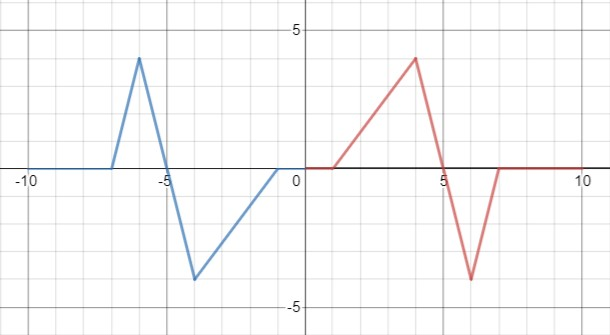
\includegraphics[width=5cm]{dAlembert_u(0,x)} }}%
\qquad
\subfloat[\centering $t=1$]{{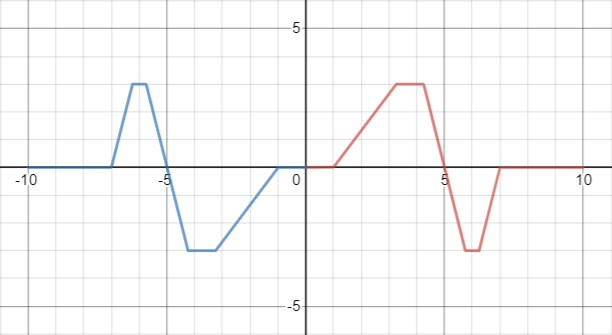
\includegraphics[width=5cm]{dAlembert_u(1,x)} }}%
\\
\subfloat[\centering $t=5$]{{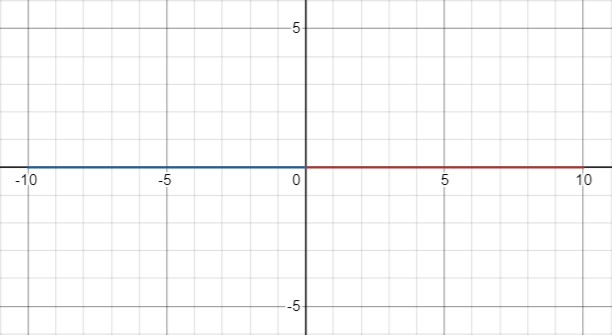
\includegraphics[width=5cm]{dAlembert_u(5,x)} }}%
\qquad
\subfloat[\centering $t=10$]{{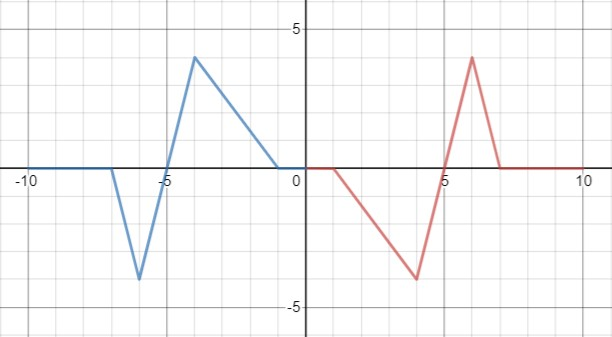
\includegraphics[width=5cm]{dAlembert_u(10,x)} }}%
\caption{Solutions to d'Alembert's formula for the given wave equation}%
\label{fig:example}%
\end{figure}
%Bibliography
\bibliography{funddiffeq}
\nocite{*}

\end{document}
